\documentclass[twoside]{book}

% Packages required by doxygen
\usepackage{fixltx2e}
\usepackage{calc}
\usepackage{doxygen}
\usepackage[export]{adjustbox} % also loads graphicx
\usepackage{graphicx}
\usepackage[utf8]{inputenc}
\usepackage{makeidx}
\usepackage{multicol}
\usepackage{multirow}
\PassOptionsToPackage{warn}{textcomp}
\usepackage{textcomp}
\usepackage[nointegrals]{wasysym}
\usepackage[table]{xcolor}

% Font selection
\usepackage[T1]{fontenc}
\usepackage[scaled=.90]{helvet}
\usepackage{courier}
\usepackage{amssymb}
\usepackage{sectsty}
\renewcommand{\familydefault}{\sfdefault}
\allsectionsfont{%
  \fontseries{bc}\selectfont%
  \color{darkgray}%
}
\renewcommand{\DoxyLabelFont}{%
  \fontseries{bc}\selectfont%
  \color{darkgray}%
}
\newcommand{\+}{\discretionary{\mbox{\scriptsize$\hookleftarrow$}}{}{}}

% Page & text layout
\usepackage{geometry}
\geometry{%
  a4paper,%
  top=2.5cm,%
  bottom=2.5cm,%
  left=2.5cm,%
  right=2.5cm%
}
\tolerance=750
\hfuzz=15pt
\hbadness=750
\setlength{\emergencystretch}{15pt}
\setlength{\parindent}{0cm}
\setlength{\parskip}{3ex plus 2ex minus 2ex}
\makeatletter
\renewcommand{\paragraph}{%
  \@startsection{paragraph}{4}{0ex}{-1.0ex}{1.0ex}{%
    \normalfont\normalsize\bfseries\SS@parafont%
  }%
}
\renewcommand{\subparagraph}{%
  \@startsection{subparagraph}{5}{0ex}{-1.0ex}{1.0ex}{%
    \normalfont\normalsize\bfseries\SS@subparafont%
  }%
}
\makeatother

% Headers & footers
\usepackage{fancyhdr}
\pagestyle{fancyplain}
\fancyhead[LE]{\fancyplain{}{\bfseries\thepage}}
\fancyhead[CE]{\fancyplain{}{}}
\fancyhead[RE]{\fancyplain{}{\bfseries\leftmark}}
\fancyhead[LO]{\fancyplain{}{\bfseries\rightmark}}
\fancyhead[CO]{\fancyplain{}{}}
\fancyhead[RO]{\fancyplain{}{\bfseries\thepage}}
\fancyfoot[LE]{\fancyplain{}{}}
\fancyfoot[CE]{\fancyplain{}{}}
\fancyfoot[RE]{\fancyplain{}{\bfseries\scriptsize Generated by Doxygen }}
\fancyfoot[LO]{\fancyplain{}{\bfseries\scriptsize Generated by Doxygen }}
\fancyfoot[CO]{\fancyplain{}{}}
\fancyfoot[RO]{\fancyplain{}{}}
\renewcommand{\footrulewidth}{0.4pt}
\renewcommand{\chaptermark}[1]{%
  \markboth{#1}{}%
}
\renewcommand{\sectionmark}[1]{%
  \markright{\thesection\ #1}%
}

% Indices & bibliography
\usepackage{natbib}
\usepackage[titles]{tocloft}
\setcounter{tocdepth}{3}
\setcounter{secnumdepth}{5}
\makeindex

% Custom commands
\newcommand{\clearemptydoublepage}{%
  \newpage{\pagestyle{empty}\cleardoublepage}%
}

\usepackage{caption}
\captionsetup{labelsep=space,justification=centering,font={bf},singlelinecheck=off,skip=4pt,position=top}

%===== C O N T E N T S =====

\begin{document}

% Titlepage & ToC
\pagenumbering{roman}
\begin{titlepage}
\vspace*{7cm}
\begin{center}%
{\Large C-\/\+Array \\[1ex]\large 0.\+1.\+3 }\\
\vspace*{1cm}
{\large Generated by Doxygen 1.8.11}\\
\end{center}
\end{titlepage}
\clearemptydoublepage
\tableofcontents
\clearemptydoublepage
\pagenumbering{arabic}

%--- Begin generated contents ---
\chapter{carray}
\label{md_README}
Python-\/like list for C 
\chapter{Module Index}
\section{Modules}
Here is a list of all modules\+:\begin{DoxyCompactList}
\item \contentsline{section}{C-\/\+Array class}{\pageref{group__carray__group}}{}
\begin{DoxyCompactList}
\item \contentsline{section}{Constants for C-\/\+Array class}{\pageref{group__cst__group}}{}
\item \contentsline{section}{Implementation specific constants and aliases}{\pageref{group__impl__group}}{}
\item \contentsline{section}{Preprocessor macros}{\pageref{group__prep__group}}{}
\item \contentsline{section}{C-\/\+Array core}{\pageref{group__core__group}}{}
\item \contentsline{section}{C-\/\+Array methods}{\pageref{group__method__group}}{}
\end{DoxyCompactList}
\end{DoxyCompactList}

\chapter{Data Structure Index}
\section{Data Structures}
Here are the data structures with brief descriptions\+:\begin{DoxyCompactList}
\item\contentsline{section}{{\bf carray} }{\pageref{structcarray}}{}
\end{DoxyCompactList}

\chapter{File Index}
\section{File List}
Here is a list of all files with brief descriptions\+:\begin{DoxyCompactList}
\item\contentsline{section}{lib/\hyperlink{cvector__core_8h}{cvector\+\_\+core.\+h} }{\pageref{cvector__core_8h}}{}
\item\contentsline{section}{lib/\hyperlink{cvector__interface_8h}{cvector\+\_\+interface.\+h} }{\pageref{cvector__interface_8h}}{}
\end{DoxyCompactList}

\chapter{Module Documentation}
\section{C-\/\+Array class}
\label{group__carray__group}\index{C-\/\+Array class@{C-\/\+Array class}}
Collaboration diagram for C-\/\+Array class\+:\nopagebreak
\begin{figure}[H]
\begin{center}
\leavevmode
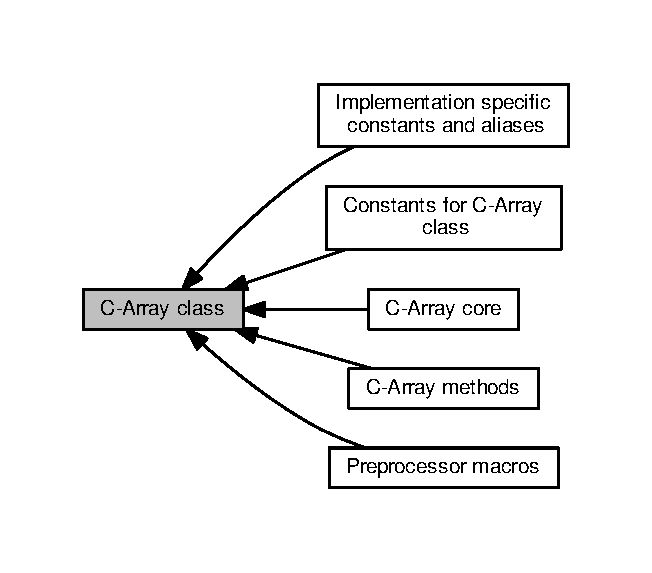
\includegraphics[width=313pt]{group__carray__group}
\end{center}
\end{figure}
\subsection*{Modules}
\begin{DoxyCompactItemize}
\item 
{\bf Constants for C-\/\+Array class}
\item 
{\bf Implementation specific constants and aliases}
\item 
{\bf Preprocessor macros}
\item 
{\bf C-\/\+Array core}
\item 
{\bf C-\/\+Array methods}
\end{DoxyCompactItemize}
\subsection*{Functions}
\begin{DoxyCompactItemize}
\item 
void {\bf fatal\+\_\+error} (char message[$\,$])
\item 
{\bf carray} $\ast$ {\bf carray\+\_\+new} ()
\item 
{\bf carray} $\ast$ {\bf carray\+\_\+new\+\_\+\+I\+SC} (size\+\_\+t init\+\_\+space)
\item 
{\bf carray} $\ast$ {\bf carray\+\_\+new\+\_\+\+CC} ({\bf carray} $\ast$copy\+\_\+carray)
\item 
{\bf carray} $\ast$ {\bf carray\+\_\+new\+\_\+\+C\+I\+SC} ({\bf carray} $\ast$copy\+\_\+carray, size\+\_\+t init\+\_\+space)
\item 
void {\bf carray\+\_\+free} ({\bf carray} $\ast$c, void($\ast$voidfunc)(type))
\item 
size\+\_\+t {\bf carray\+\_\+getsize} ({\bf carray} $\ast$c)
\item 
size\+\_\+t {\bf carray\+\_\+getspace} ({\bf carray} $\ast$c)
\item 
void {\bf carray\+\_\+setspace} ({\bf carray} $\ast$c, size\+\_\+t new\+\_\+space, void $\ast$$\ast$ok)
\item 
void {\bf carray\+\_\+addspace} ({\bf carray} $\ast$c, void $\ast$$\ast$ok)
\item 
void {\bf carray\+\_\+safeset} ({\bf carray} $\ast$c, int index, type value, void $\ast$$\ast$ok)
\item 
void {\bf carray\+\_\+append} ({\bf carray} $\ast$c, {\bf carray} $\ast$o, void $\ast$$\ast$ok)
\item 
size\+\_\+t {\bf carray\+\_\+getreadposition} ({\bf carray} $\ast$c)
\item 
void {\bf carray\+\_\+setreadposition} ({\bf carray} $\ast$c, int new\+\_\+read\+\_\+position, void $\ast$$\ast$ok)
\item 
size\+\_\+t {\bf carray\+\_\+readingsremaining} ({\bf carray} $\ast$c)
\item 
type $\ast$ {\bf carray\+\_\+getarray} ({\bf carray} $\ast$c)
\item 
type {\bf carray\+\_\+read} ({\bf carray} $\ast$c, void $\ast$$\ast$ok)
\item 
void {\bf carray\+\_\+push} ({\bf carray} $\ast$c, type value)
\item 
void {\bf carray\+\_\+ins} ({\bf carray} $\ast$c, type value)
\item 
type {\bf carray\+\_\+pop} ({\bf carray} $\ast$c)
\item 
void {\bf carray\+\_\+adjust} ({\bf carray} $\ast$c, void $\ast$$\ast$ok)
\item 
void {\bf carray\+\_\+reverse} ({\bf carray} $\ast$c)
\item 
{\bf carray} $\ast$ {\bf carray\+\_\+reversed\+\_\+\+TF} ({\bf carray} $\ast$c)
\item 
{\bf carray} $\ast$ {\bf carray\+\_\+concat\+\_\+\+TF} ({\bf carray} $\ast$a, {\bf carray} $\ast$b)
\item 
hashtype {\bf carray\+\_\+hashcode} ({\bf carray} $\ast$c, hashtype($\ast$hashfunc)(type))
\item 
bool {\bf carray\+\_\+equal} ({\bf carray} $\ast$a, {\bf carray} $\ast$b, bool($\ast$eqfunc)(type, type))
\item 
char $\ast$ {\bf carray\+\_\+tostring\+\_\+\+TF} ({\bf carray} $\ast$c, char $\ast$($\ast$strfunc)(type), char $\ast$opener, char $\ast$closer, char $\ast$prefix, char $\ast$suffix)
\item 
bool {\bf carray\+\_\+isempty} ({\bf carray} $\ast$c)
\item 
bool {\bf carray\+\_\+contains} ({\bf carray} $\ast$c, type test\+\_\+element, bool($\ast$eqfunc)(type, type))
\item 
type $\ast$ {\bf carray\+\_\+toarray\+\_\+\+TF} ({\bf carray} $\ast$c)
\item 
bool {\bf carray\+\_\+remove\+\_\+elt} ({\bf carray} $\ast$c, type test\+\_\+element, bool($\ast$eqfunc)(type, type))
\item 
void {\bf carray\+\_\+clear} ({\bf carray} $\ast$c)
\item 
type {\bf carray\+\_\+get} ({\bf carray} $\ast$c, int index, void $\ast$$\ast$ok)
\item 
void {\bf carray\+\_\+set} ({\bf carray} $\ast$c, int index, type new\+\_\+value, void $\ast$$\ast$ok)
\item 
void {\bf carray\+\_\+add} ({\bf carray} $\ast$c, int index, type new\+\_\+value, void $\ast$$\ast$ok)
\item 
type {\bf carray\+\_\+remove} ({\bf carray} $\ast$c, int index, void $\ast$$\ast$ok)
\item 
int {\bf carray\+\_\+indexof} ({\bf carray} $\ast$c, type test\+\_\+value, bool($\ast$eqfunc)(type, type))
\item 
int {\bf carray\+\_\+lastindexof} ({\bf carray} $\ast$c, type test\+\_\+value, bool($\ast$eqfunc)(type, type))
\item 
{\bf carray} $\ast$ {\bf carray\+\_\+subcarray\+\_\+\+TF} ({\bf carray} $\ast$c, int from\+\_\+index, int to\+\_\+index, void $\ast$$\ast$ok)
\item 
{\bf carray} $\ast$ {\bf carray\+\_\+subcarraystep\+\_\+\+TF} ({\bf carray} $\ast$c, int from\+\_\+index, int to\+\_\+index, int step, void $\ast$$\ast$ok)
\item 
type $\ast$ {\bf carray\+\_\+subarray\+\_\+\+TF} ({\bf carray} $\ast$c, int from\+\_\+index, int to\+\_\+index, void $\ast$$\ast$ok)
\item 
type $\ast$ {\bf carray\+\_\+subarraystep\+\_\+\+TF} ({\bf carray} $\ast$c, int from\+\_\+index, int to\+\_\+index, int step, void $\ast$$\ast$ok)
\item 
void {\bf carray\+\_\+free\+\_\+obj} (type val)
\end{DoxyCompactItemize}


\subsection{Detailed Description}


\subsection{Function Documentation}
\index{C-\/\+Array class@{C-\/\+Array class}!carray\+\_\+add@{carray\+\_\+add}}
\index{carray\+\_\+add@{carray\+\_\+add}!C-\/\+Array class@{C-\/\+Array class}}
\subsubsection[{carray\+\_\+add(carray $\ast$c, int index, type new\+\_\+value, void $\ast$$\ast$ok)}]{\setlength{\rightskip}{0pt plus 5cm}void carray\+\_\+add (
\begin{DoxyParamCaption}
\item[{{\bf carray} $\ast$}]{c, }
\item[{int}]{index, }
\item[{type}]{new\+\_\+value, }
\item[{void $\ast$$\ast$}]{ok}
\end{DoxyParamCaption}
)}\label{group__carray__group_ga121fde101d30e4885c03420658d7663f}
Adds the specified element at the specified index in the carray. If params are correct and if the operation works, ok will hold the carray address; otherwise, it will hold N\+U\+LL. 
\begin{DoxyParams}{Parameters}
{\em c} & the carray \\
\hline
{\em index} & index where to insert the specified element. The element will be inserted at this exact position, and subsequent elements will be shifted. \\
\hline
{\em new\+\_\+value} & element to insert at the specified index \\
\hline
{\em ok} & validation flag \\
\hline
\end{DoxyParams}


Definition at line 725 of file carray.\+c.

\index{C-\/\+Array class@{C-\/\+Array class}!carray\+\_\+addspace@{carray\+\_\+addspace}}
\index{carray\+\_\+addspace@{carray\+\_\+addspace}!C-\/\+Array class@{C-\/\+Array class}}
\subsubsection[{carray\+\_\+addspace(carray $\ast$c, void $\ast$$\ast$ok)}]{\setlength{\rightskip}{0pt plus 5cm}void carray\+\_\+addspace (
\begin{DoxyParamCaption}
\item[{{\bf carray} $\ast$}]{c, }
\item[{void $\ast$$\ast$}]{ok}
\end{DoxyParamCaption}
)}\label{group__carray__group_gab6421f1df72a04a6ab9780cc456ace66}
Increases space allowed for the internal representation of the carray. If params are correct and if the operation works, ok will hold the carray address; otherwise, it will hold N\+U\+LL. 
\begin{DoxyParams}{Parameters}
{\em c} & the carray \\
\hline
{\em ok} & validation flag \\
\hline
\end{DoxyParams}


Definition at line 189 of file carray.\+c.

\index{C-\/\+Array class@{C-\/\+Array class}!carray\+\_\+adjust@{carray\+\_\+adjust}}
\index{carray\+\_\+adjust@{carray\+\_\+adjust}!C-\/\+Array class@{C-\/\+Array class}}
\subsubsection[{carray\+\_\+adjust(carray $\ast$c, void $\ast$$\ast$ok)}]{\setlength{\rightskip}{0pt plus 5cm}void carray\+\_\+adjust (
\begin{DoxyParamCaption}
\item[{{\bf carray} $\ast$}]{c, }
\item[{void $\ast$$\ast$}]{ok}
\end{DoxyParamCaption}
)}\label{group__carray__group_ga2cbd4ed6aa333301a9473ce199b4dc83}
Enventually shrinks the size of the internal representation of the carray if free space exceed the threshold. ok will hold the carray address if a shrinking was made, and N\+U\+LL otherwise. 
\begin{DoxyParams}{Parameters}
{\em c} & the carray \\
\hline
{\em ok} & validation flag \\
\hline
\end{DoxyParams}


Definition at line 386 of file carray.\+c.

\index{C-\/\+Array class@{C-\/\+Array class}!carray\+\_\+append@{carray\+\_\+append}}
\index{carray\+\_\+append@{carray\+\_\+append}!C-\/\+Array class@{C-\/\+Array class}}
\subsubsection[{carray\+\_\+append(carray $\ast$c, carray $\ast$o, void $\ast$$\ast$ok)}]{\setlength{\rightskip}{0pt plus 5cm}void carray\+\_\+append (
\begin{DoxyParamCaption}
\item[{{\bf carray} $\ast$}]{c, }
\item[{{\bf carray} $\ast$}]{o, }
\item[{void $\ast$$\ast$}]{ok}
\end{DoxyParamCaption}
)}\label{group__carray__group_gad2ed91bb878032b032ed56c0c9584463}
Append the second specified carray at the end of the first one. If params are correct and if the operation works, ok will hold the carray address; otherwise, it will hold N\+U\+LL. 
\begin{DoxyParams}{Parameters}
{\em c} & the carray \\
\hline
{\em o} & the carray to put at the end of the first one \\
\hline
{\em ok} & validation flag \\
\hline
\end{DoxyParams}


Definition at line 251 of file carray.\+c.

\index{C-\/\+Array class@{C-\/\+Array class}!carray\+\_\+clear@{carray\+\_\+clear}}
\index{carray\+\_\+clear@{carray\+\_\+clear}!C-\/\+Array class@{C-\/\+Array class}}
\subsubsection[{carray\+\_\+clear(carray $\ast$c)}]{\setlength{\rightskip}{0pt plus 5cm}void carray\+\_\+clear (
\begin{DoxyParamCaption}
\item[{{\bf carray} $\ast$}]{c}
\end{DoxyParamCaption}
)}\label{group__carray__group_ga9e89ba57ce8af85ad5961d864c34397d}
Clears the content of the carray. Be careful, this function D\+O\+E\+SN\textquotesingle{}T free the space allowed for the internal representation of the carray. Use carray\+\_\+adjust for that. 
\begin{DoxyParams}{Parameters}
{\em c} & the carray \\
\hline
\end{DoxyParams}


Definition at line 652 of file carray.\+c.

\index{C-\/\+Array class@{C-\/\+Array class}!carray\+\_\+concat\+\_\+\+TF@{carray\+\_\+concat\+\_\+\+TF}}
\index{carray\+\_\+concat\+\_\+\+TF@{carray\+\_\+concat\+\_\+\+TF}!C-\/\+Array class@{C-\/\+Array class}}
\subsubsection[{carray\+\_\+concat\+\_\+\+T\+F(carray $\ast$a, carray $\ast$b)}]{\setlength{\rightskip}{0pt plus 5cm}{\bf carray}$\ast$ carray\+\_\+concat\+\_\+\+TF (
\begin{DoxyParamCaption}
\item[{{\bf carray} $\ast$}]{a, }
\item[{{\bf carray} $\ast$}]{b}
\end{DoxyParamCaption}
)}\label{group__carray__group_ga2a458a358cac5c5c070c1749f6b06571}
Concatenates both specified carrays into a new one which must be freed after use. 
\begin{DoxyParams}{Parameters}
{\em a} & the first carray to concatenate \\
\hline
{\em b} & the second carray to concatenate \\
\hline
\end{DoxyParams}
\begin{DoxyReturn}{Returns}
a concatenated version of carrays a and b 
\end{DoxyReturn}


Definition at line 438 of file carray.\+c.

\index{C-\/\+Array class@{C-\/\+Array class}!carray\+\_\+contains@{carray\+\_\+contains}}
\index{carray\+\_\+contains@{carray\+\_\+contains}!C-\/\+Array class@{C-\/\+Array class}}
\subsubsection[{carray\+\_\+contains(carray $\ast$c, type test\+\_\+element, bool($\ast$eqfunc)(type, type))}]{\setlength{\rightskip}{0pt plus 5cm}bool carray\+\_\+contains (
\begin{DoxyParamCaption}
\item[{{\bf carray} $\ast$}]{c, }
\item[{type}]{test\+\_\+element, }
\item[{bool($\ast$)(type, type)}]{eqfunc}
\end{DoxyParamCaption}
)}\label{group__carray__group_gad050a093adc14e02894e1f382c259f31}
Tests if the carray contains the test\+\_\+element according to the specified equality function 
\begin{DoxyParams}{Parameters}
{\em c} & the carray \\
\hline
{\em test\+\_\+element} & the element to be compared to the carray elements \\
\hline
{\em eqfunc} & the function to test equality between elements \\
\hline
\end{DoxyParams}
\begin{DoxyReturn}{Returns}
true if the specified element is inside the carray, and false otherwise 
\end{DoxyReturn}


Definition at line 598 of file carray.\+c.

\index{C-\/\+Array class@{C-\/\+Array class}!carray\+\_\+equal@{carray\+\_\+equal}}
\index{carray\+\_\+equal@{carray\+\_\+equal}!C-\/\+Array class@{C-\/\+Array class}}
\subsubsection[{carray\+\_\+equal(carray $\ast$a, carray $\ast$b, bool($\ast$eqfunc)(type, type))}]{\setlength{\rightskip}{0pt plus 5cm}bool carray\+\_\+equal (
\begin{DoxyParamCaption}
\item[{{\bf carray} $\ast$}]{a, }
\item[{{\bf carray} $\ast$}]{b, }
\item[{bool($\ast$)(type, type)}]{eqfunc}
\end{DoxyParamCaption}
)}\label{group__carray__group_gac243b2f9a51c9347547b4540e276a8c6}
Returns true if both carrays are equal and false otherwise, according to the specified elements equality function. 
\begin{DoxyParams}{Parameters}
{\em a} & the first carray to test \\
\hline
{\em b} & the second carray to test \\
\hline
{\em eqfunc} & equality function to apply on two elements \\
\hline
\end{DoxyParams}
\begin{DoxyReturn}{Returns}
true if both carrays are equal, false otherwise 
\end{DoxyReturn}


Definition at line 473 of file carray.\+c.

\index{C-\/\+Array class@{C-\/\+Array class}!carray\+\_\+free@{carray\+\_\+free}}
\index{carray\+\_\+free@{carray\+\_\+free}!C-\/\+Array class@{C-\/\+Array class}}
\subsubsection[{carray\+\_\+free(carray $\ast$c, void($\ast$voidfunc)(type))}]{\setlength{\rightskip}{0pt plus 5cm}void carray\+\_\+free (
\begin{DoxyParamCaption}
\item[{{\bf carray} $\ast$}]{c, }
\item[{void($\ast$)(type)}]{voidfunc}
\end{DoxyParamCaption}
)}\label{group__carray__group_ga20af624f579410d4c9de31be4d5401ec}
Destructor for carray. Frees the carray internal array representation and the carray itself. If voidfunc is not N\+U\+LL, applies this function to each element of the carray before freeing the whole struct. 
\begin{DoxyParams}{Parameters}
{\em c} & the carray \\
\hline
{\em voidfunc} & a function to be applied on each element of the carray to free it; can be N\+U\+LL \\
\hline
\end{DoxyParams}


Definition at line 120 of file carray.\+c.

\index{C-\/\+Array class@{C-\/\+Array class}!carray\+\_\+free\+\_\+obj@{carray\+\_\+free\+\_\+obj}}
\index{carray\+\_\+free\+\_\+obj@{carray\+\_\+free\+\_\+obj}!C-\/\+Array class@{C-\/\+Array class}}
\subsubsection[{carray\+\_\+free\+\_\+obj(type val)}]{\setlength{\rightskip}{0pt plus 5cm}void carray\+\_\+free\+\_\+obj (
\begin{DoxyParamCaption}
\item[{type}]{val}
\end{DoxyParamCaption}
)}\label{group__carray__group_ga36c566a87069ecd8383a02231b121c71}
Frees the specified primitive-\/wrapped element. 
\begin{DoxyParams}{Parameters}
{\em val} & primitive-\/wrapped element to free \\
\hline
\end{DoxyParams}


Definition at line 1077 of file carray.\+c.

\index{C-\/\+Array class@{C-\/\+Array class}!carray\+\_\+get@{carray\+\_\+get}}
\index{carray\+\_\+get@{carray\+\_\+get}!C-\/\+Array class@{C-\/\+Array class}}
\subsubsection[{carray\+\_\+get(carray $\ast$c, int index, void $\ast$$\ast$ok)}]{\setlength{\rightskip}{0pt plus 5cm}type carray\+\_\+get (
\begin{DoxyParamCaption}
\item[{{\bf carray} $\ast$}]{c, }
\item[{int}]{index, }
\item[{void $\ast$$\ast$}]{ok}
\end{DoxyParamCaption}
)}\label{group__carray__group_gac176f7dda1ecc9386a1e881c66e18f79}
Gets the element at the specified index in the carray. If params are correct and if the operation works, ok will hold the carray address; otherwise, it will hold N\+U\+LL. 
\begin{DoxyParams}{Parameters}
{\em c} & the carray \\
\hline
{\em index} & index where element will be retrieved \\
\hline
{\em ok} & validation flag \\
\hline
\end{DoxyParams}
\begin{DoxyReturn}{Returns}
the element at the specified index if index is correct; default type value otherwise 
\end{DoxyReturn}


Definition at line 667 of file carray.\+c.

\index{C-\/\+Array class@{C-\/\+Array class}!carray\+\_\+getarray@{carray\+\_\+getarray}}
\index{carray\+\_\+getarray@{carray\+\_\+getarray}!C-\/\+Array class@{C-\/\+Array class}}
\subsubsection[{carray\+\_\+getarray(carray $\ast$c)}]{\setlength{\rightskip}{0pt plus 5cm}type$\ast$ carray\+\_\+getarray (
\begin{DoxyParamCaption}
\item[{{\bf carray} $\ast$}]{c}
\end{DoxyParamCaption}
)}\label{group__carray__group_ga71daca172f365188a9dcd027846411a4}
Internal array getter. 
\begin{DoxyParams}{Parameters}
{\em c} & the carray \\
\hline
\end{DoxyParams}
\begin{DoxyReturn}{Returns}
the internal representation of the carray 
\end{DoxyReturn}


Definition at line 320 of file carray.\+c.

\index{C-\/\+Array class@{C-\/\+Array class}!carray\+\_\+getreadposition@{carray\+\_\+getreadposition}}
\index{carray\+\_\+getreadposition@{carray\+\_\+getreadposition}!C-\/\+Array class@{C-\/\+Array class}}
\subsubsection[{carray\+\_\+getreadposition(carray $\ast$c)}]{\setlength{\rightskip}{0pt plus 5cm}size\+\_\+t carray\+\_\+getreadposition (
\begin{DoxyParamCaption}
\item[{{\bf carray} $\ast$}]{c}
\end{DoxyParamCaption}
)}\label{group__carray__group_ga5bdf2166879f7db0ed3a65c58834ac44}
Read position getter. 
\begin{DoxyParams}{Parameters}
{\em c} & the carray \\
\hline
\end{DoxyParams}
\begin{DoxyReturn}{Returns}
the current read position 
\end{DoxyReturn}


Definition at line 276 of file carray.\+c.

\index{C-\/\+Array class@{C-\/\+Array class}!carray\+\_\+getsize@{carray\+\_\+getsize}}
\index{carray\+\_\+getsize@{carray\+\_\+getsize}!C-\/\+Array class@{C-\/\+Array class}}
\subsubsection[{carray\+\_\+getsize(carray $\ast$c)}]{\setlength{\rightskip}{0pt plus 5cm}size\+\_\+t carray\+\_\+getsize (
\begin{DoxyParamCaption}
\item[{{\bf carray} $\ast$}]{c}
\end{DoxyParamCaption}
)}\label{group__carray__group_ga1edf6d2524859ce603aa65c3525ad9ce}
Size getter. 
\begin{DoxyParams}{Parameters}
{\em c} & the carray \\
\hline
\end{DoxyParams}
\begin{DoxyReturn}{Returns}
the size of the carray 
\end{DoxyReturn}


Definition at line 138 of file carray.\+c.

\index{C-\/\+Array class@{C-\/\+Array class}!carray\+\_\+getspace@{carray\+\_\+getspace}}
\index{carray\+\_\+getspace@{carray\+\_\+getspace}!C-\/\+Array class@{C-\/\+Array class}}
\subsubsection[{carray\+\_\+getspace(carray $\ast$c)}]{\setlength{\rightskip}{0pt plus 5cm}size\+\_\+t carray\+\_\+getspace (
\begin{DoxyParamCaption}
\item[{{\bf carray} $\ast$}]{c}
\end{DoxyParamCaption}
)}\label{group__carray__group_ga4ddf3c24ac5fe16144c85aa735f94926}
Space getter. 
\begin{DoxyParams}{Parameters}
{\em c} & the carray \\
\hline
\end{DoxyParams}
\begin{DoxyReturn}{Returns}
the space (in nb of elements) of the carray 
\end{DoxyReturn}


Definition at line 148 of file carray.\+c.

\index{C-\/\+Array class@{C-\/\+Array class}!carray\+\_\+hashcode@{carray\+\_\+hashcode}}
\index{carray\+\_\+hashcode@{carray\+\_\+hashcode}!C-\/\+Array class@{C-\/\+Array class}}
\subsubsection[{carray\+\_\+hashcode(carray $\ast$c, hashtype($\ast$hashfunc)(type))}]{\setlength{\rightskip}{0pt plus 5cm}hashtype carray\+\_\+hashcode (
\begin{DoxyParamCaption}
\item[{{\bf carray} $\ast$}]{c, }
\item[{hashtype($\ast$)(type)}]{hashfunc}
\end{DoxyParamCaption}
)}\label{group__carray__group_ga36d5d46b0e74c87c694999d5924cd8ef}
Returns the hashcode of the carray according to the specified elements hash code function. 
\begin{DoxyParams}{Parameters}
{\em c} & the carray \\
\hline
{\em hashfunc} & hashcode function to apply on each element of the carray \\
\hline
\end{DoxyParams}
\begin{DoxyReturn}{Returns}
the hashcode of the carray 
\end{DoxyReturn}


Definition at line 455 of file carray.\+c.

\index{C-\/\+Array class@{C-\/\+Array class}!carray\+\_\+indexof@{carray\+\_\+indexof}}
\index{carray\+\_\+indexof@{carray\+\_\+indexof}!C-\/\+Array class@{C-\/\+Array class}}
\subsubsection[{carray\+\_\+indexof(carray $\ast$c, type test\+\_\+value, bool($\ast$eqfunc)(type, type))}]{\setlength{\rightskip}{0pt plus 5cm}int carray\+\_\+indexof (
\begin{DoxyParamCaption}
\item[{{\bf carray} $\ast$}]{c, }
\item[{type}]{test\+\_\+value, }
\item[{bool($\ast$)(type, type)}]{eqfunc}
\end{DoxyParamCaption}
)}\label{group__carray__group_ga0b9f96d48078b9b8fdbb2e8fc67393c0}
Returns the index of the specified element in the carray, and -\/1 if this element wasn\textquotesingle{}t found. The carray is read left to right and this function returns the index of the first occurence met. 
\begin{DoxyParams}{Parameters}
{\em c} & the carray \\
\hline
{\em test\+\_\+value} & the element to find in the carray \\
\hline
{\em eqfunc} & the function to test equality between elements \\
\hline
\end{DoxyParams}
\begin{DoxyReturn}{Returns}
the index of the specified element if this one was found, -\/1 otherwise 
\end{DoxyReturn}


Definition at line 813 of file carray.\+c.

\index{C-\/\+Array class@{C-\/\+Array class}!carray\+\_\+ins@{carray\+\_\+ins}}
\index{carray\+\_\+ins@{carray\+\_\+ins}!C-\/\+Array class@{C-\/\+Array class}}
\subsubsection[{carray\+\_\+ins(carray $\ast$c, type value)}]{\setlength{\rightskip}{0pt plus 5cm}void carray\+\_\+ins (
\begin{DoxyParamCaption}
\item[{{\bf carray} $\ast$}]{c, }
\item[{type}]{value}
\end{DoxyParamCaption}
)}\label{group__carray__group_ga4e7e9bd080530a6b38b9848b24036d84}
Inserts the specified value at the beginning of the carray. 
\begin{DoxyParams}{Parameters}
{\em c} & the carray \\
\hline
{\em value} & the element to insert at the end of the carray \\
\hline
\end{DoxyParams}


Definition at line 362 of file carray.\+c.

\index{C-\/\+Array class@{C-\/\+Array class}!carray\+\_\+isempty@{carray\+\_\+isempty}}
\index{carray\+\_\+isempty@{carray\+\_\+isempty}!C-\/\+Array class@{C-\/\+Array class}}
\subsubsection[{carray\+\_\+isempty(carray $\ast$c)}]{\setlength{\rightskip}{0pt plus 5cm}bool carray\+\_\+isempty (
\begin{DoxyParamCaption}
\item[{{\bf carray} $\ast$}]{c}
\end{DoxyParamCaption}
)}\label{group__carray__group_ga5ebcdfbda4ee476126a2e073702e953c}
Returns true if the carray is empty, false otherwise 
\begin{DoxyParams}{Parameters}
{\em c} & the carray \\
\hline
\end{DoxyParams}
\begin{DoxyReturn}{Returns}
true if the carray is empty, false otherwise 
\end{DoxyReturn}


Definition at line 584 of file carray.\+c.

\index{C-\/\+Array class@{C-\/\+Array class}!carray\+\_\+lastindexof@{carray\+\_\+lastindexof}}
\index{carray\+\_\+lastindexof@{carray\+\_\+lastindexof}!C-\/\+Array class@{C-\/\+Array class}}
\subsubsection[{carray\+\_\+lastindexof(carray $\ast$c, type test\+\_\+value, bool($\ast$eqfunc)(type, type))}]{\setlength{\rightskip}{0pt plus 5cm}int carray\+\_\+lastindexof (
\begin{DoxyParamCaption}
\item[{{\bf carray} $\ast$}]{c, }
\item[{type}]{test\+\_\+value, }
\item[{bool($\ast$)(type, type)}]{eqfunc}
\end{DoxyParamCaption}
)}\label{group__carray__group_ga856d0f9fc14c4a430ac24c375738de33}
Returns the index of the specified element in the carray, and -\/1 if this element wasn\textquotesingle{}t found. The carray is read right to left and this function returns the index of the first occurence met. 
\begin{DoxyParams}{Parameters}
{\em c} & the carray \\
\hline
{\em test\+\_\+value} & the element to find in the carray \\
\hline
{\em eqfunc} & the function to test equality between elements \\
\hline
\end{DoxyParams}
\begin{DoxyReturn}{Returns}
the index of the specified element if this one was found, -\/1 otherwise 
\end{DoxyReturn}


Definition at line 838 of file carray.\+c.

\index{C-\/\+Array class@{C-\/\+Array class}!carray\+\_\+new@{carray\+\_\+new}}
\index{carray\+\_\+new@{carray\+\_\+new}!C-\/\+Array class@{C-\/\+Array class}}
\subsubsection[{carray\+\_\+new()}]{\setlength{\rightskip}{0pt plus 5cm}{\bf carray}$\ast$ carray\+\_\+new (
\begin{DoxyParamCaption}
{}
\end{DoxyParamCaption}
)}\label{group__carray__group_gadab194a97d2da09dbb1ef38a1e7e06ce}
Constructor for carray. Returns a pointer to the created carray which must be freed after use. \begin{DoxyReturn}{Returns}
a pointer to the created carray 
\end{DoxyReturn}


Definition at line 37 of file carray.\+c.

\index{C-\/\+Array class@{C-\/\+Array class}!carray\+\_\+new\+\_\+\+CC@{carray\+\_\+new\+\_\+\+CC}}
\index{carray\+\_\+new\+\_\+\+CC@{carray\+\_\+new\+\_\+\+CC}!C-\/\+Array class@{C-\/\+Array class}}
\subsubsection[{carray\+\_\+new\+\_\+\+C\+C(carray $\ast$copy\+\_\+carray)}]{\setlength{\rightskip}{0pt plus 5cm}{\bf carray}$\ast$ carray\+\_\+new\+\_\+\+CC (
\begin{DoxyParamCaption}
\item[{{\bf carray} $\ast$}]{copy\+\_\+carray}
\end{DoxyParamCaption}
)}\label{group__carray__group_gafc40700f7d60a62a1967130ad5c59a24}
Copy constructor for carray. The created carray is the exact copy of the specified one with a bit more space than the length of the specified one. Returns a pointer to the created carray which must be freed after use. 
\begin{DoxyParams}{Parameters}
{\em copy\+\_\+carray} & the carray to be copied \\
\hline
\end{DoxyParams}
\begin{DoxyReturn}{Returns}
a pointer to the created carray 
\end{DoxyReturn}


Definition at line 76 of file carray.\+c.

\index{C-\/\+Array class@{C-\/\+Array class}!carray\+\_\+new\+\_\+\+C\+I\+SC@{carray\+\_\+new\+\_\+\+C\+I\+SC}}
\index{carray\+\_\+new\+\_\+\+C\+I\+SC@{carray\+\_\+new\+\_\+\+C\+I\+SC}!C-\/\+Array class@{C-\/\+Array class}}
\subsubsection[{carray\+\_\+new\+\_\+\+C\+I\+S\+C(carray $\ast$copy\+\_\+carray, size\+\_\+t init\+\_\+space)}]{\setlength{\rightskip}{0pt plus 5cm}{\bf carray}$\ast$ carray\+\_\+new\+\_\+\+C\+I\+SC (
\begin{DoxyParamCaption}
\item[{{\bf carray} $\ast$}]{copy\+\_\+carray, }
\item[{size\+\_\+t}]{init\+\_\+space}
\end{DoxyParamCaption}
)}\label{group__carray__group_ga87cf8d097d8b1c71817652226e7bcc7e}
Copy constructor for carray with init\+\_\+space specified. This carray have at least init\+\_\+space slots at instanciation, and hold the exact content of the specified carray. Returns a pointer to the created carray which must be freed after use; if init\+\_\+space is shorter than the length of the carray to be copied, returns N\+U\+LL. 
\begin{DoxyParams}{Parameters}
{\em copy\+\_\+carray} & the carray to be copied \\
\hline
{\em init\+\_\+space} & Initial space (number of elements) of the carray \\
\hline
\end{DoxyParams}
\begin{DoxyReturn}{Returns}
a pointer to the created carray 
\end{DoxyReturn}


Definition at line 97 of file carray.\+c.

\index{C-\/\+Array class@{C-\/\+Array class}!carray\+\_\+new\+\_\+\+I\+SC@{carray\+\_\+new\+\_\+\+I\+SC}}
\index{carray\+\_\+new\+\_\+\+I\+SC@{carray\+\_\+new\+\_\+\+I\+SC}!C-\/\+Array class@{C-\/\+Array class}}
\subsubsection[{carray\+\_\+new\+\_\+\+I\+S\+C(size\+\_\+t init\+\_\+space)}]{\setlength{\rightskip}{0pt plus 5cm}{\bf carray}$\ast$ carray\+\_\+new\+\_\+\+I\+SC (
\begin{DoxyParamCaption}
\item[{size\+\_\+t}]{init\+\_\+space}
\end{DoxyParamCaption}
)}\label{group__carray__group_ga97ae9c57d373662715841e97ae63029d}
Constructor for carray with specified init\+\_\+space. This carray have at least init\+\_\+space slots at instanciation. Returns a pointer to the created carray which must be freed after use; if init\+\_\+space is not valid, returns N\+U\+LL. 
\begin{DoxyParams}{Parameters}
{\em init\+\_\+space} & Initial space (number of elements) of the carray \\
\hline
\end{DoxyParams}
\begin{DoxyReturn}{Returns}
a pointer to the created carray 
\end{DoxyReturn}


Definition at line 55 of file carray.\+c.

\index{C-\/\+Array class@{C-\/\+Array class}!carray\+\_\+pop@{carray\+\_\+pop}}
\index{carray\+\_\+pop@{carray\+\_\+pop}!C-\/\+Array class@{C-\/\+Array class}}
\subsubsection[{carray\+\_\+pop(carray $\ast$c)}]{\setlength{\rightskip}{0pt plus 5cm}type carray\+\_\+pop (
\begin{DoxyParamCaption}
\item[{{\bf carray} $\ast$}]{c}
\end{DoxyParamCaption}
)}\label{group__carray__group_gac5fc202dc46c7e7fd6337cf239652625}
Removes the last element of the carray and returns it. 
\begin{DoxyParams}{Parameters}
{\em c} & the carray \\
\hline
\end{DoxyParams}
\begin{DoxyReturn}{Returns}
the last element of the carray 
\end{DoxyReturn}


Definition at line 373 of file carray.\+c.

\index{C-\/\+Array class@{C-\/\+Array class}!carray\+\_\+push@{carray\+\_\+push}}
\index{carray\+\_\+push@{carray\+\_\+push}!C-\/\+Array class@{C-\/\+Array class}}
\subsubsection[{carray\+\_\+push(carray $\ast$c, type value)}]{\setlength{\rightskip}{0pt plus 5cm}void carray\+\_\+push (
\begin{DoxyParamCaption}
\item[{{\bf carray} $\ast$}]{c, }
\item[{type}]{value}
\end{DoxyParamCaption}
)}\label{group__carray__group_gabecafdf1e57aeef8288e3a13aa174c18}
Pushes the specified value at the end of the carray. 
\begin{DoxyParams}{Parameters}
{\em c} & the carray \\
\hline
{\em value} & the element to push at the end of the carray \\
\hline
\end{DoxyParams}


Definition at line 351 of file carray.\+c.

\index{C-\/\+Array class@{C-\/\+Array class}!carray\+\_\+read@{carray\+\_\+read}}
\index{carray\+\_\+read@{carray\+\_\+read}!C-\/\+Array class@{C-\/\+Array class}}
\subsubsection[{carray\+\_\+read(carray $\ast$c, void $\ast$$\ast$ok)}]{\setlength{\rightskip}{0pt plus 5cm}type carray\+\_\+read (
\begin{DoxyParamCaption}
\item[{{\bf carray} $\ast$}]{c, }
\item[{void $\ast$$\ast$}]{ok}
\end{DoxyParamCaption}
)}\label{group__carray__group_ga7d42a90243410b19f38975b13f310410}
Read method. Returns elt at the current read position and increases read position by 1. If params are correct and if the operation works, ok will hold the carray address; otherwise, it will hold N\+U\+LL. 
\begin{DoxyParams}{Parameters}
{\em c} & the carray \\
\hline
{\em ok} & validation flag \\
\hline
\end{DoxyParams}
\begin{DoxyReturn}{Returns}
the element at the current read position; default type value if there\textquotesingle{}s no element to be read 
\end{DoxyReturn}


Definition at line 335 of file carray.\+c.

\index{C-\/\+Array class@{C-\/\+Array class}!carray\+\_\+readingsremaining@{carray\+\_\+readingsremaining}}
\index{carray\+\_\+readingsremaining@{carray\+\_\+readingsremaining}!C-\/\+Array class@{C-\/\+Array class}}
\subsubsection[{carray\+\_\+readingsremaining(carray $\ast$c)}]{\setlength{\rightskip}{0pt plus 5cm}size\+\_\+t carray\+\_\+readingsremaining (
\begin{DoxyParamCaption}
\item[{{\bf carray} $\ast$}]{c}
\end{DoxyParamCaption}
)}\label{group__carray__group_ga9aa333c655dba3f563894a56d2e06792}
Gets the number of read operation remaining before reaching the end of the carray. 
\begin{DoxyParams}{Parameters}
{\em c} & the carray \\
\hline
\end{DoxyParams}
\begin{DoxyReturn}{Returns}
the number of read possible before the end of the carray 
\end{DoxyReturn}


Definition at line 310 of file carray.\+c.

\index{C-\/\+Array class@{C-\/\+Array class}!carray\+\_\+remove@{carray\+\_\+remove}}
\index{carray\+\_\+remove@{carray\+\_\+remove}!C-\/\+Array class@{C-\/\+Array class}}
\subsubsection[{carray\+\_\+remove(carray $\ast$c, int index, void $\ast$$\ast$ok)}]{\setlength{\rightskip}{0pt plus 5cm}type carray\+\_\+remove (
\begin{DoxyParamCaption}
\item[{{\bf carray} $\ast$}]{c, }
\item[{int}]{index, }
\item[{void $\ast$$\ast$}]{ok}
\end{DoxyParamCaption}
)}\label{group__carray__group_ga92c898e128f2ae705cfaca01b3d9bb6c}
Removes the element at the specified index and returns it. If params are correct and if the operation works, ok will hold the carray address; otherwise, it will hold N\+U\+LL. 
\begin{DoxyParams}{Parameters}
{\em c} & the carray \\
\hline
{\em index} & index where element will be removed. The element will be removed at this exact position, and subsequent elements will be shifted. \\
\hline
{\em ok} & validation flag \\
\hline
\end{DoxyParams}
\begin{DoxyReturn}{Returns}
the element which have been removed if the index is correct, default type value otherwise. 
\end{DoxyReturn}


Definition at line 778 of file carray.\+c.

\index{C-\/\+Array class@{C-\/\+Array class}!carray\+\_\+remove\+\_\+elt@{carray\+\_\+remove\+\_\+elt}}
\index{carray\+\_\+remove\+\_\+elt@{carray\+\_\+remove\+\_\+elt}!C-\/\+Array class@{C-\/\+Array class}}
\subsubsection[{carray\+\_\+remove\+\_\+elt(carray $\ast$c, type test\+\_\+element, bool($\ast$eqfunc)(type, type))}]{\setlength{\rightskip}{0pt plus 5cm}bool carray\+\_\+remove\+\_\+elt (
\begin{DoxyParamCaption}
\item[{{\bf carray} $\ast$}]{c, }
\item[{type}]{test\+\_\+element, }
\item[{bool($\ast$)(type, type)}]{eqfunc}
\end{DoxyParamCaption}
)}\label{group__carray__group_ga6767be92579b30f00ab60c1a017a7a2f}
Removes the specified element from the carray if and only if this one is present. 
\begin{DoxyParams}{Parameters}
{\em c} & the carray \\
\hline
{\em test\+\_\+element} & element to be removed if present \\
\hline
{\em eqfunc} & the function to test equality between elements \\
\hline
\end{DoxyParams}
\begin{DoxyReturn}{Returns}
true if the specified element was in the carray and thus was removed, false if nothing was made. 
\end{DoxyReturn}


Definition at line 634 of file carray.\+c.

\index{C-\/\+Array class@{C-\/\+Array class}!carray\+\_\+reverse@{carray\+\_\+reverse}}
\index{carray\+\_\+reverse@{carray\+\_\+reverse}!C-\/\+Array class@{C-\/\+Array class}}
\subsubsection[{carray\+\_\+reverse(carray $\ast$c)}]{\setlength{\rightskip}{0pt plus 5cm}void carray\+\_\+reverse (
\begin{DoxyParamCaption}
\item[{{\bf carray} $\ast$}]{c}
\end{DoxyParamCaption}
)}\label{group__carray__group_gabe5aa24905e47d32ea982827a44feb0b}
Reverses the specified carray in-\/place. 
\begin{DoxyParams}{Parameters}
{\em c} & the carray \\
\hline
\end{DoxyParams}


Definition at line 402 of file carray.\+c.

\index{C-\/\+Array class@{C-\/\+Array class}!carray\+\_\+reversed\+\_\+\+TF@{carray\+\_\+reversed\+\_\+\+TF}}
\index{carray\+\_\+reversed\+\_\+\+TF@{carray\+\_\+reversed\+\_\+\+TF}!C-\/\+Array class@{C-\/\+Array class}}
\subsubsection[{carray\+\_\+reversed\+\_\+\+T\+F(carray $\ast$c)}]{\setlength{\rightskip}{0pt plus 5cm}{\bf carray}$\ast$ carray\+\_\+reversed\+\_\+\+TF (
\begin{DoxyParamCaption}
\item[{{\bf carray} $\ast$}]{c}
\end{DoxyParamCaption}
)}\label{group__carray__group_ga2b751acee4bd6b612651eb29aededf17}
Returns a reversed copy of the specified carray which must be freed after use. 
\begin{DoxyParams}{Parameters}
{\em c} & the carray \\
\hline
\end{DoxyParams}
\begin{DoxyReturn}{Returns}
a reversed copy of the specified carray 
\end{DoxyReturn}


Definition at line 419 of file carray.\+c.

\index{C-\/\+Array class@{C-\/\+Array class}!carray\+\_\+safeset@{carray\+\_\+safeset}}
\index{carray\+\_\+safeset@{carray\+\_\+safeset}!C-\/\+Array class@{C-\/\+Array class}}
\subsubsection[{carray\+\_\+safeset(carray $\ast$c, int index, type value, void $\ast$$\ast$ok)}]{\setlength{\rightskip}{0pt plus 5cm}void carray\+\_\+safeset (
\begin{DoxyParamCaption}
\item[{{\bf carray} $\ast$}]{c, }
\item[{int}]{index, }
\item[{type}]{value, }
\item[{void $\ast$$\ast$}]{ok}
\end{DoxyParamCaption}
)}\label{group__carray__group_ga9de9e3ee565848e7c850cc9968b78757}
Used to set an element somewhere in the carray even if this cell is not already used by the carray, for example, to set carray[8] with a length-\/4 carray. Unused cells until the specified one are set with the default type value. If params are correct and if the operation works, ok will hold the carray address; otherwise, it will hold N\+U\+LL. 
\begin{DoxyParams}{Parameters}
{\em c} & the carray \\
\hline
{\em index} & index where to put the specified value; can be larger than the carray size \\
\hline
{\em value} & value to be put at the specified index \\
\hline
{\em ok} & validation flag \\
\hline
\end{DoxyParams}


Definition at line 207 of file carray.\+c.

\index{C-\/\+Array class@{C-\/\+Array class}!carray\+\_\+set@{carray\+\_\+set}}
\index{carray\+\_\+set@{carray\+\_\+set}!C-\/\+Array class@{C-\/\+Array class}}
\subsubsection[{carray\+\_\+set(carray $\ast$c, int index, type new\+\_\+value, void $\ast$$\ast$ok)}]{\setlength{\rightskip}{0pt plus 5cm}void carray\+\_\+set (
\begin{DoxyParamCaption}
\item[{{\bf carray} $\ast$}]{c, }
\item[{int}]{index, }
\item[{type}]{new\+\_\+value, }
\item[{void $\ast$$\ast$}]{ok}
\end{DoxyParamCaption}
)}\label{group__carray__group_ga4345f9e37ec4fa09275465b382388c7c}
Sets the element at the specified index in the carray to the specified value. If params are correct and if the operation works, ok will hold the carray address; otherwise, it will hold N\+U\+LL. 
\begin{DoxyParams}{Parameters}
{\em c} & the carray \\
\hline
{\em index} & index where element will be set \\
\hline
{\em new\+\_\+value} & new value for this element \\
\hline
{\em ok} & validation flag \\
\hline
\end{DoxyParams}


Definition at line 697 of file carray.\+c.

\index{C-\/\+Array class@{C-\/\+Array class}!carray\+\_\+setreadposition@{carray\+\_\+setreadposition}}
\index{carray\+\_\+setreadposition@{carray\+\_\+setreadposition}!C-\/\+Array class@{C-\/\+Array class}}
\subsubsection[{carray\+\_\+setreadposition(carray $\ast$c, int new\+\_\+read\+\_\+position, void $\ast$$\ast$ok)}]{\setlength{\rightskip}{0pt plus 5cm}void carray\+\_\+setreadposition (
\begin{DoxyParamCaption}
\item[{{\bf carray} $\ast$}]{c, }
\item[{int}]{new\+\_\+read\+\_\+position, }
\item[{void $\ast$$\ast$}]{ok}
\end{DoxyParamCaption}
)}\label{group__carray__group_ga758790318888562ef72e8044b6382cc8}
Read position setter. If params are correct and if the operation works, ok will hold the carray address; otherwise, it will hold N\+U\+LL. 
\begin{DoxyParams}{Parameters}
{\em c} & the carray \\
\hline
{\em new\+\_\+read\+\_\+position} & new read position \\
\hline
{\em ok} & validation flag \\
\hline
\end{DoxyParams}


Definition at line 289 of file carray.\+c.

\index{C-\/\+Array class@{C-\/\+Array class}!carray\+\_\+setspace@{carray\+\_\+setspace}}
\index{carray\+\_\+setspace@{carray\+\_\+setspace}!C-\/\+Array class@{C-\/\+Array class}}
\subsubsection[{carray\+\_\+setspace(carray $\ast$c, size\+\_\+t new\+\_\+space, void $\ast$$\ast$ok)}]{\setlength{\rightskip}{0pt plus 5cm}void carray\+\_\+setspace (
\begin{DoxyParamCaption}
\item[{{\bf carray} $\ast$}]{c, }
\item[{size\+\_\+t}]{new\+\_\+space, }
\item[{void $\ast$$\ast$}]{ok}
\end{DoxyParamCaption}
)}\label{group__carray__group_ga480c374470da1c2657cbdd6d5d84e63b}
Space setter. Can be used to modify the space allowed for the internal representation of the carray. If params are correct and if the operation works, ok will hold the carray address; otherwise, it will hold N\+U\+LL. 
\begin{DoxyParams}{Parameters}
{\em c} & the carray \\
\hline
{\em new\+\_\+space} & new space (in nb of elements) for the carray \\
\hline
{\em validation} & flag \\
\hline
\end{DoxyParams}


Definition at line 162 of file carray.\+c.

\index{C-\/\+Array class@{C-\/\+Array class}!carray\+\_\+subarray\+\_\+\+TF@{carray\+\_\+subarray\+\_\+\+TF}}
\index{carray\+\_\+subarray\+\_\+\+TF@{carray\+\_\+subarray\+\_\+\+TF}!C-\/\+Array class@{C-\/\+Array class}}
\subsubsection[{carray\+\_\+subarray\+\_\+\+T\+F(carray $\ast$c, int from\+\_\+index, int to\+\_\+index, void $\ast$$\ast$ok)}]{\setlength{\rightskip}{0pt plus 5cm}type$\ast$ carray\+\_\+subarray\+\_\+\+TF (
\begin{DoxyParamCaption}
\item[{{\bf carray} $\ast$}]{c, }
\item[{int}]{from\+\_\+index, }
\item[{int}]{to\+\_\+index, }
\item[{void $\ast$$\ast$}]{ok}
\end{DoxyParamCaption}
)}\label{group__carray__group_ga812c846b20b687b1e7a61d0ae672f405}
Returns a smaller vanilla array which holds values from index \char`\"{}from\+\_\+index\char`\"{} (included) to index \char`\"{}to\+\_\+index\char`\"{} (excluded). If params are correct and if the operation works, ok will hold the carray address; otherwise, it will hold N\+U\+LL. 
\begin{DoxyParams}{Parameters}
{\em c} & the carray \\
\hline
{\em from\+\_\+index} & beginning index \\
\hline
{\em to\+\_\+index} & ending index \\
\hline
{\em ok} & validation flag \\
\hline
\end{DoxyParams}
\begin{DoxyReturn}{Returns}
the sub-\/vanilla array if the indices are correct, N\+U\+LL otherwise 
\end{DoxyReturn}


Definition at line 977 of file carray.\+c.

\index{C-\/\+Array class@{C-\/\+Array class}!carray\+\_\+subarraystep\+\_\+\+TF@{carray\+\_\+subarraystep\+\_\+\+TF}}
\index{carray\+\_\+subarraystep\+\_\+\+TF@{carray\+\_\+subarraystep\+\_\+\+TF}!C-\/\+Array class@{C-\/\+Array class}}
\subsubsection[{carray\+\_\+subarraystep\+\_\+\+T\+F(carray $\ast$c, int from\+\_\+index, int to\+\_\+index, int step, void $\ast$$\ast$ok)}]{\setlength{\rightskip}{0pt plus 5cm}type$\ast$ carray\+\_\+subarraystep\+\_\+\+TF (
\begin{DoxyParamCaption}
\item[{{\bf carray} $\ast$}]{c, }
\item[{int}]{from\+\_\+index, }
\item[{int}]{to\+\_\+index, }
\item[{int}]{step, }
\item[{void $\ast$$\ast$}]{ok}
\end{DoxyParamCaption}
)}\label{group__carray__group_ga7b9044937f80d9bbc1b6b348434f7e12}
Returns a smaller vanilla array which holds values from index \char`\"{}from\+\_\+index\char`\"{} (included) to index \char`\"{}to\+\_\+index\char`\"{} (excluded) according to the specified step. If params are correct and if the operation works, ok will hold the carray address; otherwise, it will hold N\+U\+LL. 
\begin{DoxyParams}{Parameters}
{\em c} & the carray \\
\hline
{\em from\+\_\+index} & beginning index \\
\hline
{\em to\+\_\+index} & ending index \\
\hline
{\em step} & item selecting step \\
\hline
{\em ok} & validation flag \\
\hline
\end{DoxyParams}
\begin{DoxyReturn}{Returns}
the sub-\/vanilla array if the indices are correct, N\+U\+LL otherwise 
\end{DoxyReturn}


Definition at line 1019 of file carray.\+c.

\index{C-\/\+Array class@{C-\/\+Array class}!carray\+\_\+subcarray\+\_\+\+TF@{carray\+\_\+subcarray\+\_\+\+TF}}
\index{carray\+\_\+subcarray\+\_\+\+TF@{carray\+\_\+subcarray\+\_\+\+TF}!C-\/\+Array class@{C-\/\+Array class}}
\subsubsection[{carray\+\_\+subcarray\+\_\+\+T\+F(carray $\ast$c, int from\+\_\+index, int to\+\_\+index, void $\ast$$\ast$ok)}]{\setlength{\rightskip}{0pt plus 5cm}{\bf carray}$\ast$ carray\+\_\+subcarray\+\_\+\+TF (
\begin{DoxyParamCaption}
\item[{{\bf carray} $\ast$}]{c, }
\item[{int}]{from\+\_\+index, }
\item[{int}]{to\+\_\+index, }
\item[{void $\ast$$\ast$}]{ok}
\end{DoxyParamCaption}
)}\label{group__carray__group_ga678ec7aaf616a13739dd7bd07af8156d}
Returns a smaller carray which holds values from index \char`\"{}from\+\_\+index\char`\"{} (included) to index \char`\"{}to\+\_\+index\char`\"{} (excluded). If params are correct and if the operation works, ok will hold the carray address; otherwise, it will hold N\+U\+LL. 
\begin{DoxyParams}{Parameters}
{\em c} & the carray \\
\hline
{\em from\+\_\+index} & beginning index \\
\hline
{\em to\+\_\+index} & ending index \\
\hline
{\em ok} & validation flag \\
\hline
\end{DoxyParams}
\begin{DoxyReturn}{Returns}
the sub-\/carray if the indices are correct, N\+U\+LL otherwise 
\end{DoxyReturn}


Definition at line 864 of file carray.\+c.

\index{C-\/\+Array class@{C-\/\+Array class}!carray\+\_\+subcarraystep\+\_\+\+TF@{carray\+\_\+subcarraystep\+\_\+\+TF}}
\index{carray\+\_\+subcarraystep\+\_\+\+TF@{carray\+\_\+subcarraystep\+\_\+\+TF}!C-\/\+Array class@{C-\/\+Array class}}
\subsubsection[{carray\+\_\+subcarraystep\+\_\+\+T\+F(carray $\ast$c, int from\+\_\+index, int to\+\_\+index, int step, void $\ast$$\ast$ok)}]{\setlength{\rightskip}{0pt plus 5cm}{\bf carray}$\ast$ carray\+\_\+subcarraystep\+\_\+\+TF (
\begin{DoxyParamCaption}
\item[{{\bf carray} $\ast$}]{c, }
\item[{int}]{from\+\_\+index, }
\item[{int}]{to\+\_\+index, }
\item[{int}]{step, }
\item[{void $\ast$$\ast$}]{ok}
\end{DoxyParamCaption}
)}\label{group__carray__group_ga256bc6acdc6c7e7065d6fd68fbd794b5}
Returns a smaller carray which holds values from index \char`\"{}from\+\_\+index\char`\"{} (included) to index \char`\"{}to\+\_\+index\char`\"{} (excluded) according to the specified step. If params are correct and if the operation works, ok will hold the carray address; otherwise, it will hold N\+U\+LL. 
\begin{DoxyParams}{Parameters}
{\em c} & the carray \\
\hline
{\em from\+\_\+index} & beginning index \\
\hline
{\em to\+\_\+index} & ending index \\
\hline
{\em step} & item selecting step \\
\hline
{\em ok} & validation flag \\
\hline
\end{DoxyParams}
\begin{DoxyReturn}{Returns}
the sub-\/carray if the indices are correct, N\+U\+LL otherwise 
\end{DoxyReturn}


Definition at line 908 of file carray.\+c.

\index{C-\/\+Array class@{C-\/\+Array class}!carray\+\_\+toarray\+\_\+\+TF@{carray\+\_\+toarray\+\_\+\+TF}}
\index{carray\+\_\+toarray\+\_\+\+TF@{carray\+\_\+toarray\+\_\+\+TF}!C-\/\+Array class@{C-\/\+Array class}}
\subsubsection[{carray\+\_\+toarray\+\_\+\+T\+F(carray $\ast$c)}]{\setlength{\rightskip}{0pt plus 5cm}type$\ast$ carray\+\_\+toarray\+\_\+\+TF (
\begin{DoxyParamCaption}
\item[{{\bf carray} $\ast$}]{c}
\end{DoxyParamCaption}
)}\label{group__carray__group_ga13d1ba5db9dd55b7dccbe9c223c4ec49}
Returns a vanilla array version of the carray. 
\begin{DoxyParams}{Parameters}
{\em c} & the carray \\
\hline
\end{DoxyParams}
\begin{DoxyReturn}{Returns}
a vanilla array version of the carray 
\end{DoxyReturn}


Definition at line 618 of file carray.\+c.

\index{C-\/\+Array class@{C-\/\+Array class}!carray\+\_\+tostring\+\_\+\+TF@{carray\+\_\+tostring\+\_\+\+TF}}
\index{carray\+\_\+tostring\+\_\+\+TF@{carray\+\_\+tostring\+\_\+\+TF}!C-\/\+Array class@{C-\/\+Array class}}
\subsubsection[{carray\+\_\+tostring\+\_\+\+T\+F(carray $\ast$c, char $\ast$($\ast$strfunc)(type), char $\ast$opener, char $\ast$closer, char $\ast$prefix, char $\ast$suffix)}]{\setlength{\rightskip}{0pt plus 5cm}char$\ast$ carray\+\_\+tostring\+\_\+\+TF (
\begin{DoxyParamCaption}
\item[{{\bf carray} $\ast$}]{c, }
\item[{char $\ast$($\ast$)(type)}]{strfunc, }
\item[{char $\ast$}]{opener, }
\item[{char $\ast$}]{closer, }
\item[{char $\ast$}]{prefix, }
\item[{char $\ast$}]{suffix}
\end{DoxyParamCaption}
)}\label{group__carray__group_gaf5c05493fb356a0039939a74ac15ac1a}
Returns a representation of the specified carray. 
\begin{DoxyParams}{Parameters}
{\em c} & the carray \\
\hline
{\em strfunc} & the function to apply on each element to convert it into string \\
\hline
{\em opener} & opening string \\
\hline
{\em closer} & closing string \\
\hline
{\em prefix} & prefix string added before each cell except for the first one \\
\hline
{\em suffix} & suffix string added after each cell except for the lats one \\
\hline
\end{DoxyParams}
\begin{DoxyReturn}{Returns}
a string representing the carray 
\end{DoxyReturn}


Definition at line 500 of file carray.\+c.

\index{C-\/\+Array class@{C-\/\+Array class}!fatal\+\_\+error@{fatal\+\_\+error}}
\index{fatal\+\_\+error@{fatal\+\_\+error}!C-\/\+Array class@{C-\/\+Array class}}
\subsubsection[{fatal\+\_\+error(char message[])}]{\setlength{\rightskip}{0pt plus 5cm}void fatal\+\_\+error (
\begin{DoxyParamCaption}
\item[{char}]{message[$\,$]}
\end{DoxyParamCaption}
)}\label{group__carray__group_ga4caf39c943223eb36313986b87a2645b}
Prints an error message 
\begin{DoxyParams}{Parameters}
{\em message} & message to print \\
\hline
\end{DoxyParams}


Definition at line 27 of file carray.\+c.


\section{Constants for C-\/\+Array class}
\label{group__cst__group}\index{Constants for C-\/\+Array class@{Constants for C-\/\+Array class}}
Collaboration diagram for Constants for C-\/\+Array class\+:\nopagebreak
\begin{figure}[H]
\begin{center}
\leavevmode
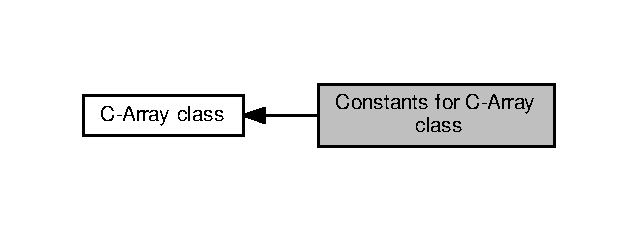
\includegraphics[width=306pt]{group__cst__group}
\end{center}
\end{figure}
\subsection*{Macros}
\begin{DoxyCompactItemize}
\item 
\#define {\bf D\+E\+F\+A\+U\+L\+T\+\_\+\+S\+P\+A\+C\+E\+\_\+\+I\+N\+I\+T\+\_\+\+F\+L\+AT}~8
\item 
\#define {\bf D\+E\+F\+A\+U\+L\+T\+\_\+\+S\+P\+A\+C\+E\+\_\+\+I\+N\+I\+T\+\_\+\+P\+E\+R\+C\+E\+NT}~1.\+25
\item 
\#define {\bf D\+E\+F\+A\+U\+L\+T\+\_\+\+S\+P\+A\+C\+E\+\_\+\+I\+N\+CR}~2.\+0
\item 
\#define {\bf D\+E\+F\+A\+U\+L\+T\+\_\+\+S\+H\+R\+I\+N\+K\+\_\+\+T\+H\+R\+E\+S\+H\+O\+LD}~2.\+5
\item 
\#define {\bf D\+E\+F\+A\+U\+L\+T\+\_\+\+S\+H\+R\+I\+N\+K\+\_\+\+P\+E\+R\+C\+E\+NT}~1.\+25
\end{DoxyCompactItemize}
\subsection*{Typedefs}
\begin{DoxyCompactItemize}
\item 
typedef struct {\bf carray} {\bf carray}
\end{DoxyCompactItemize}


\subsection{Detailed Description}


\subsection{Macro Definition Documentation}
\index{Constants for C-\/\+Array class@{Constants for C-\/\+Array class}!D\+E\+F\+A\+U\+L\+T\+\_\+\+S\+H\+R\+I\+N\+K\+\_\+\+P\+E\+R\+C\+E\+NT@{D\+E\+F\+A\+U\+L\+T\+\_\+\+S\+H\+R\+I\+N\+K\+\_\+\+P\+E\+R\+C\+E\+NT}}
\index{D\+E\+F\+A\+U\+L\+T\+\_\+\+S\+H\+R\+I\+N\+K\+\_\+\+P\+E\+R\+C\+E\+NT@{D\+E\+F\+A\+U\+L\+T\+\_\+\+S\+H\+R\+I\+N\+K\+\_\+\+P\+E\+R\+C\+E\+NT}!Constants for C-\/\+Array class@{Constants for C-\/\+Array class}}
\subsubsection[{D\+E\+F\+A\+U\+L\+T\+\_\+\+S\+H\+R\+I\+N\+K\+\_\+\+P\+E\+R\+C\+E\+NT}]{\setlength{\rightskip}{0pt plus 5cm}\#define D\+E\+F\+A\+U\+L\+T\+\_\+\+S\+H\+R\+I\+N\+K\+\_\+\+P\+E\+R\+C\+E\+NT~1.\+25}\label{group__cst__group_ga157ceedbc7cfdd92a7bc50015720d130}
Space factor used when the carray is shrinked. 

Definition at line 50 of file carray.\+h.

\index{Constants for C-\/\+Array class@{Constants for C-\/\+Array class}!D\+E\+F\+A\+U\+L\+T\+\_\+\+S\+H\+R\+I\+N\+K\+\_\+\+T\+H\+R\+E\+S\+H\+O\+LD@{D\+E\+F\+A\+U\+L\+T\+\_\+\+S\+H\+R\+I\+N\+K\+\_\+\+T\+H\+R\+E\+S\+H\+O\+LD}}
\index{D\+E\+F\+A\+U\+L\+T\+\_\+\+S\+H\+R\+I\+N\+K\+\_\+\+T\+H\+R\+E\+S\+H\+O\+LD@{D\+E\+F\+A\+U\+L\+T\+\_\+\+S\+H\+R\+I\+N\+K\+\_\+\+T\+H\+R\+E\+S\+H\+O\+LD}!Constants for C-\/\+Array class@{Constants for C-\/\+Array class}}
\subsubsection[{D\+E\+F\+A\+U\+L\+T\+\_\+\+S\+H\+R\+I\+N\+K\+\_\+\+T\+H\+R\+E\+S\+H\+O\+LD}]{\setlength{\rightskip}{0pt plus 5cm}\#define D\+E\+F\+A\+U\+L\+T\+\_\+\+S\+H\+R\+I\+N\+K\+\_\+\+T\+H\+R\+E\+S\+H\+O\+LD~2.\+5}\label{group__cst__group_gad333b0148b725977097636f9d20cafbe}
Space threshold from which the carray is shrinked. 

Definition at line 45 of file carray.\+h.

\index{Constants for C-\/\+Array class@{Constants for C-\/\+Array class}!D\+E\+F\+A\+U\+L\+T\+\_\+\+S\+P\+A\+C\+E\+\_\+\+I\+N\+CR@{D\+E\+F\+A\+U\+L\+T\+\_\+\+S\+P\+A\+C\+E\+\_\+\+I\+N\+CR}}
\index{D\+E\+F\+A\+U\+L\+T\+\_\+\+S\+P\+A\+C\+E\+\_\+\+I\+N\+CR@{D\+E\+F\+A\+U\+L\+T\+\_\+\+S\+P\+A\+C\+E\+\_\+\+I\+N\+CR}!Constants for C-\/\+Array class@{Constants for C-\/\+Array class}}
\subsubsection[{D\+E\+F\+A\+U\+L\+T\+\_\+\+S\+P\+A\+C\+E\+\_\+\+I\+N\+CR}]{\setlength{\rightskip}{0pt plus 5cm}\#define D\+E\+F\+A\+U\+L\+T\+\_\+\+S\+P\+A\+C\+E\+\_\+\+I\+N\+CR~2.\+0}\label{group__cst__group_ga7cd586c1ea2e214b7e382bf8761cfdca}
Space factor used when a carray becomes too short. 

Definition at line 40 of file carray.\+h.

\index{Constants for C-\/\+Array class@{Constants for C-\/\+Array class}!D\+E\+F\+A\+U\+L\+T\+\_\+\+S\+P\+A\+C\+E\+\_\+\+I\+N\+I\+T\+\_\+\+F\+L\+AT@{D\+E\+F\+A\+U\+L\+T\+\_\+\+S\+P\+A\+C\+E\+\_\+\+I\+N\+I\+T\+\_\+\+F\+L\+AT}}
\index{D\+E\+F\+A\+U\+L\+T\+\_\+\+S\+P\+A\+C\+E\+\_\+\+I\+N\+I\+T\+\_\+\+F\+L\+AT@{D\+E\+F\+A\+U\+L\+T\+\_\+\+S\+P\+A\+C\+E\+\_\+\+I\+N\+I\+T\+\_\+\+F\+L\+AT}!Constants for C-\/\+Array class@{Constants for C-\/\+Array class}}
\subsubsection[{D\+E\+F\+A\+U\+L\+T\+\_\+\+S\+P\+A\+C\+E\+\_\+\+I\+N\+I\+T\+\_\+\+F\+L\+AT}]{\setlength{\rightskip}{0pt plus 5cm}\#define D\+E\+F\+A\+U\+L\+T\+\_\+\+S\+P\+A\+C\+E\+\_\+\+I\+N\+I\+T\+\_\+\+F\+L\+AT~8}\label{group__cst__group_ga6f95be98bc9d7df0405a2ab712470941}
Initial space for the internal representation of a carray. 

Definition at line 30 of file carray.\+h.

\index{Constants for C-\/\+Array class@{Constants for C-\/\+Array class}!D\+E\+F\+A\+U\+L\+T\+\_\+\+S\+P\+A\+C\+E\+\_\+\+I\+N\+I\+T\+\_\+\+P\+E\+R\+C\+E\+NT@{D\+E\+F\+A\+U\+L\+T\+\_\+\+S\+P\+A\+C\+E\+\_\+\+I\+N\+I\+T\+\_\+\+P\+E\+R\+C\+E\+NT}}
\index{D\+E\+F\+A\+U\+L\+T\+\_\+\+S\+P\+A\+C\+E\+\_\+\+I\+N\+I\+T\+\_\+\+P\+E\+R\+C\+E\+NT@{D\+E\+F\+A\+U\+L\+T\+\_\+\+S\+P\+A\+C\+E\+\_\+\+I\+N\+I\+T\+\_\+\+P\+E\+R\+C\+E\+NT}!Constants for C-\/\+Array class@{Constants for C-\/\+Array class}}
\subsubsection[{D\+E\+F\+A\+U\+L\+T\+\_\+\+S\+P\+A\+C\+E\+\_\+\+I\+N\+I\+T\+\_\+\+P\+E\+R\+C\+E\+NT}]{\setlength{\rightskip}{0pt plus 5cm}\#define D\+E\+F\+A\+U\+L\+T\+\_\+\+S\+P\+A\+C\+E\+\_\+\+I\+N\+I\+T\+\_\+\+P\+E\+R\+C\+E\+NT~1.\+25}\label{group__cst__group_gad53e382c777b098aee95e2b065b722f5}
Initial space factor used when a carray is created from an existing one. 

Definition at line 35 of file carray.\+h.



\subsection{Typedef Documentation}
\index{Constants for C-\/\+Array class@{Constants for C-\/\+Array class}!carray@{carray}}
\index{carray@{carray}!Constants for C-\/\+Array class@{Constants for C-\/\+Array class}}
\subsubsection[{carray}]{\setlength{\rightskip}{0pt plus 5cm}typedef struct {\bf carray} {\bf carray}}\label{group__cst__group_ga1555d5c8eff5c3672cfb92c56fe5a776}
Alias for carray struct. 

Definition at line 55 of file carray.\+h.


\section{Implementation specific constants and aliases}
\label{group__impl__group}\index{Implementation specific constants and aliases@{Implementation specific constants and aliases}}
Collaboration diagram for Implementation specific constants and aliases\+:\nopagebreak
\begin{figure}[H]
\begin{center}
\leavevmode
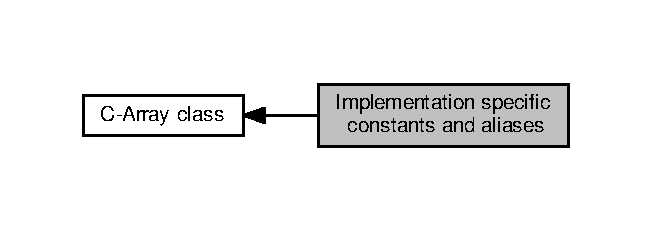
\includegraphics[width=313pt]{group__impl__group}
\end{center}
\end{figure}
\subsection*{Macros}
\begin{DoxyCompactItemize}
\item 
\#define {\bfseries P\+R\+I\+M\+E\+\_\+\+C\+ST}~31\label{group__impl__group_ga123c33de7154c282b66935373832c3d2}

\item 
\#define {\bfseries D\+E\+F\+A\+U\+L\+T\+\_\+\+T\+Y\+P\+E\+\_\+\+V\+A\+L\+UE}~N\+U\+LL\label{group__impl__group_ga48b008dd6b494f297c36976dbefde3a6}

\end{DoxyCompactItemize}
\subsection*{Typedefs}
\begin{DoxyCompactItemize}
\item 
typedef unsigned int {\bfseries hashtype}\label{group__impl__group_ga666aae09a1f6137dd5f36f54b7f0551f}

\item 
typedef void $\ast$ {\bfseries type}\label{group__impl__group_ga00adf28a743db83fba0f44c7533f8395}

\end{DoxyCompactItemize}


\subsection{Detailed Description}

\section{Preprocessor macros}
\label{group__prep__group}\index{Preprocessor macros@{Preprocessor macros}}
Collaboration diagram for Preprocessor macros\+:\nopagebreak
\begin{figure}[H]
\begin{center}
\leavevmode
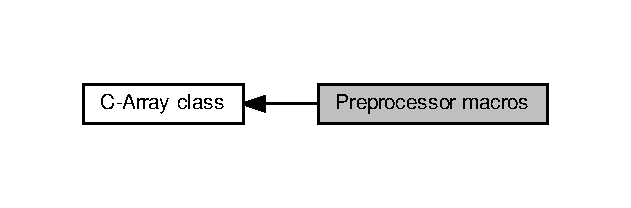
\includegraphics[width=303pt]{group__prep__group}
\end{center}
\end{figure}
\subsection*{Macros}
\begin{DoxyCompactItemize}
\item 
\#define {\bfseries of\+\_\+\+Char}~$\ast$(char$\ast$)\label{group__prep__group_gabcfcd74817919703a130dbc1cbb57bed}

\item 
\#define {\bfseries of\+\_\+s\+Char}~$\ast$(signed char$\ast$)\label{group__prep__group_ga679d07007e61761bec873e67f0aa26ea}

\item 
\#define {\bfseries of\+\_\+u\+Char}~$\ast$(unsigned char$\ast$)\label{group__prep__group_gaa123653b9114c4bdc3e5394ffe390aa9}

\item 
\#define {\bfseries of\+\_\+\+Short}~$\ast$(short$\ast$)\label{group__prep__group_ga29102bbb7c49380c032672464d0c21b1}

\item 
\#define {\bfseries of\+\_\+s\+Short}~$\ast$(signed short$\ast$)\label{group__prep__group_ga6144058541f159966bbb43c15ef6eb16}

\item 
\#define {\bfseries of\+\_\+u\+Short}~$\ast$(unsigned short$\ast$)\label{group__prep__group_ga9a7b4f128c834c336c604c4967b3ae05}

\item 
\#define {\bfseries of\+\_\+\+Int}~$\ast$(int$\ast$)\label{group__prep__group_gad13bbd80bfa8a4b060b0c3c8ee8b4593}

\item 
\#define {\bfseries of\+\_\+s\+Int}~$\ast$(signed int$\ast$)\label{group__prep__group_gab44ba54e2338cf1fafc7d27f896b7015}

\item 
\#define {\bfseries of\+\_\+u\+Int}~$\ast$(unsigned int$\ast$)\label{group__prep__group_ga8bf6641d75fd9053261a16bb6b2caf0a}

\item 
\#define {\bfseries of\+\_\+\+Long}~$\ast$(long$\ast$)\label{group__prep__group_gae44e91d7b6ae86e944ae0bbaa99833ae}

\item 
\#define {\bfseries of\+\_\+l\+Long}~$\ast$(long long$\ast$)\label{group__prep__group_gac6b50729853f98250eac5019393be709}

\item 
\#define {\bfseries of\+\_\+s\+Long}~$\ast$(signed long$\ast$)\label{group__prep__group_gabf4d5db51a66d2f32d406a38b6658fd4}

\item 
\#define {\bfseries of\+\_\+sl\+Long}~$\ast$(signed long long$\ast$)\label{group__prep__group_gabd16ef323cea08f78278d94e7afc9a96}

\item 
\#define {\bfseries of\+\_\+u\+Long}~$\ast$(unsigned long$\ast$)\label{group__prep__group_ga90a21dace6a26e9621c450c457d1de75}

\item 
\#define {\bfseries of\+\_\+ul\+Long}~$\ast$(unsigned long long$\ast$)\label{group__prep__group_ga3e7eebc5340362dc526a7e88d5ceba6a}

\item 
\#define {\bfseries of\+\_\+\+Float}~$\ast$(float$\ast$)\label{group__prep__group_gafe0bc3592b5f8c7eb00d0cc1a329400a}

\item 
\#define {\bfseries of\+\_\+\+Double}~$\ast$(double$\ast$)\label{group__prep__group_ga6b0f1440a5eafde45f7de6e3fe5bc0a1}

\item 
\#define {\bfseries of\+\_\+l\+Double}~$\ast$(long double$\ast$)\label{group__prep__group_gacd514a033626484b018828fbf1dafcde}

\item 
\#define {\bfseries of\+\_\+\+Bool}~$\ast$(bool$\ast$)\label{group__prep__group_gaf998c625df8bb0979492bdc6331e7cf5}

\item 
\#define {\bfseries of\+\_\+\+String}~(char$\ast$)\label{group__prep__group_ga905845e335099d8083b3db6e92615ae0}

\item 
\#define {\bfseries Char}(expr)
\item 
\#define {\bfseries s\+Char}(expr)
\item 
\#define {\bfseries u\+Char}(expr)
\item 
\#define {\bfseries Short}(expr)
\item 
\#define {\bfseries s\+Short}(expr)
\item 
\#define {\bfseries u\+Short}(expr)
\item 
\#define {\bfseries Int}(expr)
\item 
\#define {\bfseries s\+Int}(expr)
\item 
\#define {\bfseries u\+Int}(expr)
\item 
\#define {\bfseries Long}(expr)
\item 
\#define {\bfseries l\+Long}(expr)
\item 
\#define {\bfseries s\+Long}(expr)
\item 
\#define {\bfseries sl\+Long}(expr)
\item 
\#define {\bfseries u\+Long}(expr)
\item 
\#define {\bfseries ul\+Long}(expr)
\item 
\#define {\bfseries Float}(expr)
\item 
\#define {\bfseries Double}(expr)
\item 
\#define {\bfseries l\+Double}(expr)
\item 
\#define {\bfseries Bool}(expr)
\item 
\#define {\bfseries String}(expr)
\item 
\#define {\bfseries free\+\_\+\+Obj}~\&{\bf carray\+\_\+free\+\_\+obj}\label{group__prep__group_ga7d141aff3ea5c308d91ba1d75d82910c}

\end{DoxyCompactItemize}
\subsection*{Functions}
\begin{DoxyCompactItemize}
\item 
void {\bf carray\+\_\+free\+\_\+obj} (type)
\end{DoxyCompactItemize}
\subsection*{Variables}
\begin{DoxyCompactItemize}
\item 
char $\ast$ {\bfseries Char\+\_\+holder}\label{group__prep__group_ga6c28268b220bf8963e9d83ab3ea4e1fc}

\item 
signed char $\ast$ {\bfseries s\+Char\+\_\+holder}\label{group__prep__group_ga2952cc9f34c30813a61bbf448687cb37}

\item 
unsigned char $\ast$ {\bfseries u\+Char\+\_\+holder}\label{group__prep__group_ga515997135a9fd60f330e7c80ba35e4a3}

\item 
short $\ast$ {\bfseries Short\+\_\+holder}\label{group__prep__group_ga50dfd89c93ee41c7a4d361449ff54b66}

\item 
signed short $\ast$ {\bfseries s\+Short\+\_\+holder}\label{group__prep__group_gae5801f872635cae195d49f253976bafb}

\item 
unsigned short $\ast$ {\bfseries u\+Short\+\_\+holder}\label{group__prep__group_ga44eb5e51833f5adb71a5566f4c044947}

\item 
int $\ast$ {\bfseries Int\+\_\+holder}\label{group__prep__group_gae717b1cf30ad00b04f5e492ade36bacc}

\item 
signed int $\ast$ {\bfseries s\+Int\+\_\+holder}\label{group__prep__group_ga7fdea5b2401ae8217aa51cfef7965452}

\item 
unsigned int $\ast$ {\bfseries u\+Int\+\_\+holder}\label{group__prep__group_ga5d873117ab0bcac78e1c027843f5c813}

\item 
long $\ast$ {\bfseries Long\+\_\+holder}\label{group__prep__group_ga5684531bd7fc7624b968eb17b2fe961a}

\item 
long long $\ast$ {\bfseries l\+Long\+\_\+holder}\label{group__prep__group_ga71901a53a2dd9764340602973b0a9102}

\item 
signed long $\ast$ {\bfseries s\+Long\+\_\+holder}\label{group__prep__group_ga14f3d44ac57e9e7d5f06d1fba4fc32b6}

\item 
signed long long $\ast$ {\bfseries sl\+Long\+\_\+holder}\label{group__prep__group_ga3edb914eb9f50e1aab83523cdaea35b5}

\item 
unsigned long $\ast$ {\bfseries u\+Long\+\_\+holder}\label{group__prep__group_ga4baf95556984d597b0b0e0de6c2aaf97}

\item 
unsigned long long $\ast$ {\bfseries ul\+Long\+\_\+holder}\label{group__prep__group_gab4ac89b39be6dbdb6e08853fec2c2960}

\item 
float $\ast$ {\bfseries Float\+\_\+holder}\label{group__prep__group_gac18354ce9886c8f92111cc797e32e895}

\item 
double $\ast$ {\bfseries Double\+\_\+holder}\label{group__prep__group_ga936ba5ce64968cd5a1a235e31338be7a}

\item 
long double $\ast$ {\bfseries l\+Double\+\_\+holder}\label{group__prep__group_ga97e6637c976a858407ce778841c83839}

\item 
bool $\ast$ {\bfseries Bool\+\_\+holder}\label{group__prep__group_gad4dbdeac7a57b51e62851b6eb71ad71c}

\item 
char $\ast$ {\bfseries String\+\_\+holder}\label{group__prep__group_ga2edc7e7c4249c98033ba2846a0ed435b}

\end{DoxyCompactItemize}


\subsection{Detailed Description}


\subsection{Macro Definition Documentation}
\index{Preprocessor macros@{Preprocessor macros}!Bool@{Bool}}
\index{Bool@{Bool}!Preprocessor macros@{Preprocessor macros}}
\subsubsection[{Bool}]{\setlength{\rightskip}{0pt plus 5cm}\#define Bool(
\begin{DoxyParamCaption}
\item[{}]{expr}
\end{DoxyParamCaption}
)}\label{group__prep__group_gad2d944f0b88aa92abb7ab4cbd4178adc}
{\bfseries Value\+:}
\begin{DoxyCode}
(Bool\_holder = malloc(\textcolor{keyword}{sizeof}(\textcolor{keywordtype}{bool})), \(\backslash\)
     *Bool\_holder = (expr), Bool\_holder)
\end{DoxyCode}


Definition at line 189 of file carray.\+h.

\index{Preprocessor macros@{Preprocessor macros}!Char@{Char}}
\index{Char@{Char}!Preprocessor macros@{Preprocessor macros}}
\subsubsection[{Char}]{\setlength{\rightskip}{0pt plus 5cm}\#define Char(
\begin{DoxyParamCaption}
\item[{}]{expr}
\end{DoxyParamCaption}
)}\label{group__prep__group_ga342a65d86a563cd2ea540447fc3e5521}
{\bfseries Value\+:}
\begin{DoxyCode}
(Char\_holder = malloc(\textcolor{keyword}{sizeof}(\textcolor{keywordtype}{char})), \(\backslash\)
     *Char\_holder = (expr), Char\_holder)
\end{DoxyCode}


Definition at line 99 of file carray.\+h.

\index{Preprocessor macros@{Preprocessor macros}!Double@{Double}}
\index{Double@{Double}!Preprocessor macros@{Preprocessor macros}}
\subsubsection[{Double}]{\setlength{\rightskip}{0pt plus 5cm}\#define Double(
\begin{DoxyParamCaption}
\item[{}]{expr}
\end{DoxyParamCaption}
)}\label{group__prep__group_gaa158a13c81272a98d092c2a8d65d677b}
{\bfseries Value\+:}
\begin{DoxyCode}
(Double\_holder = malloc(\textcolor{keyword}{sizeof}(\textcolor{keywordtype}{double})), \(\backslash\)
     *Double\_holder = (expr), Double\_holder)
\end{DoxyCode}


Definition at line 179 of file carray.\+h.

\index{Preprocessor macros@{Preprocessor macros}!Float@{Float}}
\index{Float@{Float}!Preprocessor macros@{Preprocessor macros}}
\subsubsection[{Float}]{\setlength{\rightskip}{0pt plus 5cm}\#define Float(
\begin{DoxyParamCaption}
\item[{}]{expr}
\end{DoxyParamCaption}
)}\label{group__prep__group_gad868402b314334a308258e1fd067c920}
{\bfseries Value\+:}
\begin{DoxyCode}
(Float\_holder = malloc(\textcolor{keyword}{sizeof}(\textcolor{keywordtype}{float})), \(\backslash\)
     *Float\_holder = (expr), Float\_holder)
\end{DoxyCode}


Definition at line 174 of file carray.\+h.

\index{Preprocessor macros@{Preprocessor macros}!Int@{Int}}
\index{Int@{Int}!Preprocessor macros@{Preprocessor macros}}
\subsubsection[{Int}]{\setlength{\rightskip}{0pt plus 5cm}\#define Int(
\begin{DoxyParamCaption}
\item[{}]{expr}
\end{DoxyParamCaption}
)}\label{group__prep__group_gaeb37b787ef316604a51c61ded9859d97}
{\bfseries Value\+:}
\begin{DoxyCode}
(Int\_holder = malloc(\textcolor{keyword}{sizeof}(\textcolor{keywordtype}{int})), \(\backslash\)
     *Int\_holder = (expr), Int\_holder)
\end{DoxyCode}


Definition at line 129 of file carray.\+h.

\index{Preprocessor macros@{Preprocessor macros}!l\+Double@{l\+Double}}
\index{l\+Double@{l\+Double}!Preprocessor macros@{Preprocessor macros}}
\subsubsection[{l\+Double}]{\setlength{\rightskip}{0pt plus 5cm}\#define l\+Double(
\begin{DoxyParamCaption}
\item[{}]{expr}
\end{DoxyParamCaption}
)}\label{group__prep__group_ga1dc5528b4b59e30e8fe8a873685182c3}
{\bfseries Value\+:}
\begin{DoxyCode}
(lDouble\_holder = malloc(\textcolor{keyword}{sizeof}(\textcolor{keywordtype}{long} \textcolor{keywordtype}{double})), \(\backslash\)
     *lDouble\_holder = (expr), lDouble\_holder)
\end{DoxyCode}


Definition at line 184 of file carray.\+h.

\index{Preprocessor macros@{Preprocessor macros}!l\+Long@{l\+Long}}
\index{l\+Long@{l\+Long}!Preprocessor macros@{Preprocessor macros}}
\subsubsection[{l\+Long}]{\setlength{\rightskip}{0pt plus 5cm}\#define l\+Long(
\begin{DoxyParamCaption}
\item[{}]{expr}
\end{DoxyParamCaption}
)}\label{group__prep__group_ga8b1da64b8027b082faedbbaa7239b41d}
{\bfseries Value\+:}
\begin{DoxyCode}
(lLong\_holder = malloc(\textcolor{keyword}{sizeof}(\textcolor{keywordtype}{long} \textcolor{keywordtype}{long})), \(\backslash\)
     *lLong\_holder = (expr), lLong\_holder)
\end{DoxyCode}


Definition at line 149 of file carray.\+h.

\index{Preprocessor macros@{Preprocessor macros}!Long@{Long}}
\index{Long@{Long}!Preprocessor macros@{Preprocessor macros}}
\subsubsection[{Long}]{\setlength{\rightskip}{0pt plus 5cm}\#define Long(
\begin{DoxyParamCaption}
\item[{}]{expr}
\end{DoxyParamCaption}
)}\label{group__prep__group_ga9f55426e31eadefd7e636570deb85779}
{\bfseries Value\+:}
\begin{DoxyCode}
(Long\_holder = malloc(\textcolor{keyword}{sizeof}(\textcolor{keywordtype}{long})), \(\backslash\)
     *Long\_holder = (expr), Long\_holder)
\end{DoxyCode}


Definition at line 144 of file carray.\+h.

\index{Preprocessor macros@{Preprocessor macros}!s\+Char@{s\+Char}}
\index{s\+Char@{s\+Char}!Preprocessor macros@{Preprocessor macros}}
\subsubsection[{s\+Char}]{\setlength{\rightskip}{0pt plus 5cm}\#define s\+Char(
\begin{DoxyParamCaption}
\item[{}]{expr}
\end{DoxyParamCaption}
)}\label{group__prep__group_gaf08aad63815e83bacfa9317564b2bc41}
{\bfseries Value\+:}
\begin{DoxyCode}
(sChar\_holder = malloc(\textcolor{keyword}{sizeof}(\textcolor{keywordtype}{signed} \textcolor{keywordtype}{char})), \(\backslash\)
     *sChar\_holder = (expr), sChar\_holder)
\end{DoxyCode}


Definition at line 104 of file carray.\+h.

\index{Preprocessor macros@{Preprocessor macros}!Short@{Short}}
\index{Short@{Short}!Preprocessor macros@{Preprocessor macros}}
\subsubsection[{Short}]{\setlength{\rightskip}{0pt plus 5cm}\#define Short(
\begin{DoxyParamCaption}
\item[{}]{expr}
\end{DoxyParamCaption}
)}\label{group__prep__group_gaf75f4e0ca317aa3fe5bcb84cca980c0e}
{\bfseries Value\+:}
\begin{DoxyCode}
(Short\_holder = malloc(\textcolor{keyword}{sizeof}(\textcolor{keywordtype}{short})), \(\backslash\)
     *Short\_holder = (expr), Short\_holder)
\end{DoxyCode}


Definition at line 114 of file carray.\+h.

\index{Preprocessor macros@{Preprocessor macros}!s\+Int@{s\+Int}}
\index{s\+Int@{s\+Int}!Preprocessor macros@{Preprocessor macros}}
\subsubsection[{s\+Int}]{\setlength{\rightskip}{0pt plus 5cm}\#define s\+Int(
\begin{DoxyParamCaption}
\item[{}]{expr}
\end{DoxyParamCaption}
)}\label{group__prep__group_gabdac3861f88ca1f6c3a9724fcf1e4b35}
{\bfseries Value\+:}
\begin{DoxyCode}
(sInt\_holder = malloc(\textcolor{keyword}{sizeof}(\textcolor{keywordtype}{signed} \textcolor{keywordtype}{int})), \(\backslash\)
     *sInt\_holder = (expr), sInt\_holder)
\end{DoxyCode}


Definition at line 134 of file carray.\+h.

\index{Preprocessor macros@{Preprocessor macros}!sl\+Long@{sl\+Long}}
\index{sl\+Long@{sl\+Long}!Preprocessor macros@{Preprocessor macros}}
\subsubsection[{sl\+Long}]{\setlength{\rightskip}{0pt plus 5cm}\#define sl\+Long(
\begin{DoxyParamCaption}
\item[{}]{expr}
\end{DoxyParamCaption}
)}\label{group__prep__group_ga83f39e6139a6907ff20ac51ab694f2c6}
{\bfseries Value\+:}
\begin{DoxyCode}
(slLong\_holder = malloc(\textcolor{keyword}{sizeof}(\textcolor{keywordtype}{signed} \textcolor{keywordtype}{long} \textcolor{keywordtype}{long})), \(\backslash\)
     *slLong\_holder = (expr), slLong\_holder)
\end{DoxyCode}


Definition at line 159 of file carray.\+h.

\index{Preprocessor macros@{Preprocessor macros}!s\+Long@{s\+Long}}
\index{s\+Long@{s\+Long}!Preprocessor macros@{Preprocessor macros}}
\subsubsection[{s\+Long}]{\setlength{\rightskip}{0pt plus 5cm}\#define s\+Long(
\begin{DoxyParamCaption}
\item[{}]{expr}
\end{DoxyParamCaption}
)}\label{group__prep__group_gaeb3124a63adf934b56c8beaf5f24e543}
{\bfseries Value\+:}
\begin{DoxyCode}
(sLong\_holder = malloc(\textcolor{keyword}{sizeof}(\textcolor{keywordtype}{signed} \textcolor{keywordtype}{long})), \(\backslash\)
     *sLong\_holder = (expr), sLong\_holder)
\end{DoxyCode}


Definition at line 154 of file carray.\+h.

\index{Preprocessor macros@{Preprocessor macros}!s\+Short@{s\+Short}}
\index{s\+Short@{s\+Short}!Preprocessor macros@{Preprocessor macros}}
\subsubsection[{s\+Short}]{\setlength{\rightskip}{0pt plus 5cm}\#define s\+Short(
\begin{DoxyParamCaption}
\item[{}]{expr}
\end{DoxyParamCaption}
)}\label{group__prep__group_ga8b7d6af879bc0fe6454bc2bc4a243a0d}
{\bfseries Value\+:}
\begin{DoxyCode}
(sShort\_holder = malloc(\textcolor{keyword}{sizeof}(\textcolor{keywordtype}{signed} \textcolor{keywordtype}{short})), \(\backslash\)
     *sShort\_holder = (expr), sShort\_holder)
\end{DoxyCode}


Definition at line 119 of file carray.\+h.

\index{Preprocessor macros@{Preprocessor macros}!String@{String}}
\index{String@{String}!Preprocessor macros@{Preprocessor macros}}
\subsubsection[{String}]{\setlength{\rightskip}{0pt plus 5cm}\#define String(
\begin{DoxyParamCaption}
\item[{}]{expr}
\end{DoxyParamCaption}
)}\label{group__prep__group_ga2a0b6a5a39b256067af8893d4fe1cac4}
{\bfseries Value\+:}
\begin{DoxyCode}
(String\_holder = malloc(\textcolor{keyword}{sizeof}(expr) / \textcolor{keyword}{sizeof}(\textcolor{keywordtype}{char})), \(\backslash\)
     strcpy(String\_holder, (expr)), \(\backslash\)
     String\_holder)
\end{DoxyCode}


Definition at line 194 of file carray.\+h.

\index{Preprocessor macros@{Preprocessor macros}!u\+Char@{u\+Char}}
\index{u\+Char@{u\+Char}!Preprocessor macros@{Preprocessor macros}}
\subsubsection[{u\+Char}]{\setlength{\rightskip}{0pt plus 5cm}\#define u\+Char(
\begin{DoxyParamCaption}
\item[{}]{expr}
\end{DoxyParamCaption}
)}\label{group__prep__group_ga18cb2e7b24f75ab4fa7dd68b2a8f3c8a}
{\bfseries Value\+:}
\begin{DoxyCode}
(uChar\_holder = malloc(\textcolor{keyword}{sizeof}(\textcolor{keywordtype}{unsigned} \textcolor{keywordtype}{char})), \(\backslash\)
     *uChar\_holder = (expr), uChar\_holder)
\end{DoxyCode}


Definition at line 109 of file carray.\+h.

\index{Preprocessor macros@{Preprocessor macros}!u\+Int@{u\+Int}}
\index{u\+Int@{u\+Int}!Preprocessor macros@{Preprocessor macros}}
\subsubsection[{u\+Int}]{\setlength{\rightskip}{0pt plus 5cm}\#define u\+Int(
\begin{DoxyParamCaption}
\item[{}]{expr}
\end{DoxyParamCaption}
)}\label{group__prep__group_ga3a521600a57e10d664b0544043a134a4}
{\bfseries Value\+:}
\begin{DoxyCode}
(uInt\_holder = malloc(\textcolor{keyword}{sizeof}(\textcolor{keywordtype}{unsigned} \textcolor{keywordtype}{int})), \(\backslash\)
     *uInt\_holder = (expr), uInt\_holder)
\end{DoxyCode}


Definition at line 139 of file carray.\+h.

\index{Preprocessor macros@{Preprocessor macros}!ul\+Long@{ul\+Long}}
\index{ul\+Long@{ul\+Long}!Preprocessor macros@{Preprocessor macros}}
\subsubsection[{ul\+Long}]{\setlength{\rightskip}{0pt plus 5cm}\#define ul\+Long(
\begin{DoxyParamCaption}
\item[{}]{expr}
\end{DoxyParamCaption}
)}\label{group__prep__group_ga59d8ce4d3e125e6717c81c41fe2855f3}
{\bfseries Value\+:}
\begin{DoxyCode}
(ulLong\_holder = malloc(\textcolor{keyword}{sizeof}(\textcolor{keywordtype}{unsigned} \textcolor{keywordtype}{long} \textcolor{keywordtype}{long})), \(\backslash\)
     *ulLong\_holder = (expr), ulLong\_holder)
\end{DoxyCode}


Definition at line 169 of file carray.\+h.

\index{Preprocessor macros@{Preprocessor macros}!u\+Long@{u\+Long}}
\index{u\+Long@{u\+Long}!Preprocessor macros@{Preprocessor macros}}
\subsubsection[{u\+Long}]{\setlength{\rightskip}{0pt plus 5cm}\#define u\+Long(
\begin{DoxyParamCaption}
\item[{}]{expr}
\end{DoxyParamCaption}
)}\label{group__prep__group_ga178bb442d01dda1ceb7b7dbe871fcb77}
{\bfseries Value\+:}
\begin{DoxyCode}
(uLong\_holder = malloc(\textcolor{keyword}{sizeof}(\textcolor{keywordtype}{unsigned} \textcolor{keywordtype}{long})), \(\backslash\)
     *uLong\_holder = (expr), uLong\_holder)
\end{DoxyCode}


Definition at line 164 of file carray.\+h.

\index{Preprocessor macros@{Preprocessor macros}!u\+Short@{u\+Short}}
\index{u\+Short@{u\+Short}!Preprocessor macros@{Preprocessor macros}}
\subsubsection[{u\+Short}]{\setlength{\rightskip}{0pt plus 5cm}\#define u\+Short(
\begin{DoxyParamCaption}
\item[{}]{expr}
\end{DoxyParamCaption}
)}\label{group__prep__group_ga619de1dcb6be13a12778f0f532d86483}
{\bfseries Value\+:}
\begin{DoxyCode}
(uShort\_holder = malloc(\textcolor{keyword}{sizeof}(\textcolor{keywordtype}{unsigned} \textcolor{keywordtype}{short})), \(\backslash\)
     *uShort\_holder = (expr), uShort\_holder)
\end{DoxyCode}


Definition at line 124 of file carray.\+h.



\subsection{Function Documentation}
\index{Preprocessor macros@{Preprocessor macros}!carray\+\_\+free\+\_\+obj@{carray\+\_\+free\+\_\+obj}}
\index{carray\+\_\+free\+\_\+obj@{carray\+\_\+free\+\_\+obj}!Preprocessor macros@{Preprocessor macros}}
\subsubsection[{carray\+\_\+free\+\_\+obj(type)}]{\setlength{\rightskip}{0pt plus 5cm}void carray\+\_\+free\+\_\+obj (
\begin{DoxyParamCaption}
\item[{type}]{val}
\end{DoxyParamCaption}
)}\label{group__prep__group_gaa983dcd204e02b0ae6b7dab25ab0e03f}
Frees the specified primitive-\/wrapped element. 
\begin{DoxyParams}{Parameters}
{\em val} & primitive-\/wrapped element to free \\
\hline
\end{DoxyParams}


Definition at line 1077 of file carray.\+c.


\section{C-\/\+Array core}
\label{group__core__group}\index{C-\/\+Array core@{C-\/\+Array core}}
Collaboration diagram for C-\/\+Array core\+:\nopagebreak
\begin{figure}[H]
\begin{center}
\leavevmode
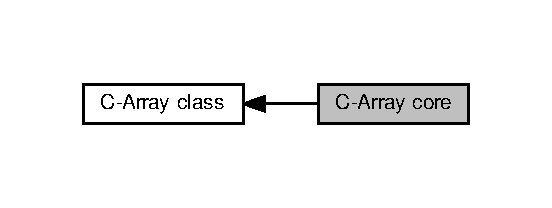
\includegraphics[width=265pt]{group__core__group}
\end{center}
\end{figure}
\subsection*{Data Structures}
\begin{DoxyCompactItemize}
\item 
struct {\bf carray}
\end{DoxyCompactItemize}


\subsection{Detailed Description}

\section{C-\/\+Array methods}
\label{group__method__group}\index{C-\/\+Array methods@{C-\/\+Array methods}}
Collaboration diagram for C-\/\+Array methods\+:\nopagebreak
\begin{figure}[H]
\begin{center}
\leavevmode
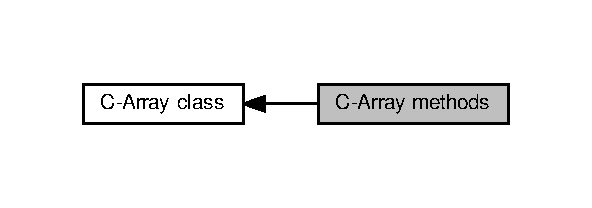
\includegraphics[width=284pt]{group__method__group}
\end{center}
\end{figure}
\subsection*{Functions}
\begin{DoxyCompactItemize}
\item 
{\bf carray} $\ast$ {\bf carray\+\_\+new} ()
\item 
{\bf carray} $\ast$ {\bf carray\+\_\+new\+\_\+\+I\+SC} (size\+\_\+t)
\item 
{\bf carray} $\ast$ {\bf carray\+\_\+new\+\_\+\+CC} ({\bf carray} $\ast$)
\item 
{\bf carray} $\ast$ {\bf carray\+\_\+new\+\_\+\+C\+I\+SC} ({\bf carray} $\ast$, size\+\_\+t)
\item 
void {\bfseries carray\+\_\+free} ({\bf carray} $\ast$, void(type))\label{group__method__group_ga07e0bf89d4437f8fe81c79101c3ca92c}

\item 
size\+\_\+t {\bf carray\+\_\+getsize} ({\bf carray} $\ast$)
\item 
void {\bf carray\+\_\+clear} ({\bf carray} $\ast$)
\item 
bool {\bf carray\+\_\+isempty} ({\bf carray} $\ast$)
\item 
size\+\_\+t {\bf carray\+\_\+getspace} ({\bf carray} $\ast$)
\item 
void {\bf carray\+\_\+setspace} ({\bf carray} $\ast$, size\+\_\+t, void $\ast$$\ast$)
\item 
void {\bf carray\+\_\+adjust} ({\bf carray} $\ast$, void $\ast$$\ast$)
\item 
size\+\_\+t {\bf carray\+\_\+getreadposition} ({\bf carray} $\ast$)
\item 
size\+\_\+t {\bf carray\+\_\+readingsremaining} ({\bf carray} $\ast$)
\item 
void {\bf carray\+\_\+setreadposition} ({\bf carray} $\ast$, int, void $\ast$$\ast$)
\item 
type $\ast$ {\bf carray\+\_\+getarray} ({\bf carray} $\ast$)
\item 
type {\bf carray\+\_\+read} ({\bf carray} $\ast$, void $\ast$$\ast$ok)
\item 
void {\bf carray\+\_\+reverse} ({\bf carray} $\ast$)
\item 
{\bf carray} $\ast$ {\bf carray\+\_\+reversed\+\_\+\+TF} ({\bf carray} $\ast$)
\item 
void {\bf carray\+\_\+append} ({\bf carray} $\ast$, {\bf carray} $\ast$, void $\ast$$\ast$)
\item 
{\bf carray} $\ast$ {\bf carray\+\_\+concat\+\_\+\+TF} ({\bf carray} $\ast$, {\bf carray} $\ast$)
\item 
char $\ast$ {\bfseries carray\+\_\+tostring\+\_\+\+TF} ({\bf carray} $\ast$, char $\ast$(type), char $\ast$, char $\ast$, char $\ast$, char $\ast$)\label{group__method__group_ga8c5907136724e99dc8212d9c333ab027}

\item 
hashtype {\bfseries carray\+\_\+hashcode} ({\bf carray} $\ast$, hashtype(type))\label{group__method__group_gab6fce3c1883194f7b4e298d108249b00}

\item 
bool {\bfseries carray\+\_\+equal} ({\bf carray} $\ast$, {\bf carray} $\ast$, bool(type, type))\label{group__method__group_gaccb5ee3de6441dcf90e5ae9c214d6858}

\item 
int {\bfseries carray\+\_\+indexof} ({\bf carray} $\ast$, type, bool(type, type))\label{group__method__group_ga097246bae1483f9b0aec8fed166a2ba5}

\item 
int {\bfseries carray\+\_\+lastindexof} ({\bf carray} $\ast$, type, bool(type, type))\label{group__method__group_ga322e73429a9d78339367f844d5aa74cd}

\item 
bool {\bfseries carray\+\_\+contains} ({\bf carray} $\ast$, type, bool(type, type))\label{group__method__group_gac98417b7832e24a9aa15ef44681b728e}

\item 
{\bf carray} $\ast$ {\bf carray\+\_\+subcarray\+\_\+\+TF} ({\bf carray} $\ast$, int, int, void $\ast$$\ast$)
\item 
{\bf carray} $\ast$ {\bf carray\+\_\+subcarraystep\+\_\+\+TF} ({\bf carray} $\ast$, int, int, int, void $\ast$$\ast$)
\item 
type $\ast$ {\bf carray\+\_\+subarray\+\_\+\+TF} ({\bf carray} $\ast$, int, int, void $\ast$$\ast$)
\item 
type $\ast$ {\bf carray\+\_\+subarraystep\+\_\+\+TF} ({\bf carray} $\ast$, int, int, int, void $\ast$$\ast$)
\item 
type $\ast$ {\bf carray\+\_\+toarray\+\_\+\+TF} ({\bf carray} $\ast$)
\item 
type {\bf carray\+\_\+get} ({\bf carray} $\ast$, int, void $\ast$$\ast$)
\item 
void {\bf carray\+\_\+add} ({\bf carray} $\ast$, int, type, void $\ast$$\ast$)
\item 
void {\bf carray\+\_\+push} ({\bf carray} $\ast$, type)
\item 
void {\bf carray\+\_\+ins} ({\bf carray} $\ast$, type)
\item 
void {\bf carray\+\_\+set} ({\bf carray} $\ast$, int, type, void $\ast$$\ast$)
\item 
void {\bf carray\+\_\+safeset} ({\bf carray} $\ast$, int, type, void $\ast$$\ast$)
\item 
type {\bf carray\+\_\+remove} ({\bf carray} $\ast$, int, void $\ast$$\ast$)
\item 
type {\bf carray\+\_\+pop} ({\bf carray} $\ast$)
\item 
bool {\bfseries carray\+\_\+remove\+\_\+elt} ({\bf carray} $\ast$, type, bool(type, type))\label{group__method__group_gaf0547e1fd95952667b22f433485ad7fd}

\end{DoxyCompactItemize}


\subsection{Detailed Description}


\subsection{Function Documentation}
\index{C-\/\+Array methods@{C-\/\+Array methods}!carray\+\_\+add@{carray\+\_\+add}}
\index{carray\+\_\+add@{carray\+\_\+add}!C-\/\+Array methods@{C-\/\+Array methods}}
\subsubsection[{carray\+\_\+add(carray $\ast$, int, type, void $\ast$$\ast$)}]{\setlength{\rightskip}{0pt plus 5cm}void carray\+\_\+add (
\begin{DoxyParamCaption}
\item[{{\bf carray} $\ast$}]{c, }
\item[{int}]{index, }
\item[{type}]{new\+\_\+value, }
\item[{void $\ast$$\ast$}]{ok}
\end{DoxyParamCaption}
)}\label{group__method__group_ga7007ad6008499ca9362a9201aa61fa4d}
Adds the specified element at the specified index in the carray. If params are correct and if the operation works, ok will hold the carray address; otherwise, it will hold N\+U\+LL. 
\begin{DoxyParams}{Parameters}
{\em c} & the carray \\
\hline
{\em index} & index where to insert the specified element. The element will be inserted at this exact position, and subsequent elements will be shifted. \\
\hline
{\em new\+\_\+value} & element to insert at the specified index \\
\hline
{\em ok} & validation flag \\
\hline
\end{DoxyParams}


Definition at line 725 of file carray.\+c.

\index{C-\/\+Array methods@{C-\/\+Array methods}!carray\+\_\+adjust@{carray\+\_\+adjust}}
\index{carray\+\_\+adjust@{carray\+\_\+adjust}!C-\/\+Array methods@{C-\/\+Array methods}}
\subsubsection[{carray\+\_\+adjust(carray $\ast$, void $\ast$$\ast$)}]{\setlength{\rightskip}{0pt plus 5cm}void carray\+\_\+adjust (
\begin{DoxyParamCaption}
\item[{{\bf carray} $\ast$}]{c, }
\item[{void $\ast$$\ast$}]{ok}
\end{DoxyParamCaption}
)}\label{group__method__group_ga0539a588e5172e5d7bcdb8ff8a4c60e1}
Enventually shrinks the size of the internal representation of the carray if free space exceed the threshold. ok will hold the carray address if a shrinking was made, and N\+U\+LL otherwise. 
\begin{DoxyParams}{Parameters}
{\em c} & the carray \\
\hline
{\em ok} & validation flag \\
\hline
\end{DoxyParams}


Definition at line 386 of file carray.\+c.

\index{C-\/\+Array methods@{C-\/\+Array methods}!carray\+\_\+append@{carray\+\_\+append}}
\index{carray\+\_\+append@{carray\+\_\+append}!C-\/\+Array methods@{C-\/\+Array methods}}
\subsubsection[{carray\+\_\+append(carray $\ast$, carray $\ast$, void $\ast$$\ast$)}]{\setlength{\rightskip}{0pt plus 5cm}void carray\+\_\+append (
\begin{DoxyParamCaption}
\item[{{\bf carray} $\ast$}]{c, }
\item[{{\bf carray} $\ast$}]{o, }
\item[{void $\ast$$\ast$}]{ok}
\end{DoxyParamCaption}
)}\label{group__method__group_ga49f7fa113929359b84a5bdd6987674b7}
Append the second specified carray at the end of the first one. If params are correct and if the operation works, ok will hold the carray address; otherwise, it will hold N\+U\+LL. 
\begin{DoxyParams}{Parameters}
{\em c} & the carray \\
\hline
{\em o} & the carray to put at the end of the first one \\
\hline
{\em ok} & validation flag \\
\hline
\end{DoxyParams}


Definition at line 251 of file carray.\+c.

\index{C-\/\+Array methods@{C-\/\+Array methods}!carray\+\_\+clear@{carray\+\_\+clear}}
\index{carray\+\_\+clear@{carray\+\_\+clear}!C-\/\+Array methods@{C-\/\+Array methods}}
\subsubsection[{carray\+\_\+clear(carray $\ast$)}]{\setlength{\rightskip}{0pt plus 5cm}void carray\+\_\+clear (
\begin{DoxyParamCaption}
\item[{{\bf carray} $\ast$}]{c}
\end{DoxyParamCaption}
)}\label{group__method__group_ga19dffa556ed3cf5bbabe82559d80057f}
Clears the content of the carray. Be careful, this function D\+O\+E\+SN\textquotesingle{}T free the space allowed for the internal representation of the carray. Use carray\+\_\+adjust for that. 
\begin{DoxyParams}{Parameters}
{\em c} & the carray \\
\hline
\end{DoxyParams}


Definition at line 652 of file carray.\+c.

\index{C-\/\+Array methods@{C-\/\+Array methods}!carray\+\_\+concat\+\_\+\+TF@{carray\+\_\+concat\+\_\+\+TF}}
\index{carray\+\_\+concat\+\_\+\+TF@{carray\+\_\+concat\+\_\+\+TF}!C-\/\+Array methods@{C-\/\+Array methods}}
\subsubsection[{carray\+\_\+concat\+\_\+\+T\+F(carray $\ast$, carray $\ast$)}]{\setlength{\rightskip}{0pt plus 5cm}{\bf carray}$\ast$ carray\+\_\+concat\+\_\+\+TF (
\begin{DoxyParamCaption}
\item[{{\bf carray} $\ast$}]{a, }
\item[{{\bf carray} $\ast$}]{b}
\end{DoxyParamCaption}
)}\label{group__method__group_gadb3f6f5b18c2178abf1be668b3d99786}
Concatenates both specified carrays into a new one which must be freed after use. 
\begin{DoxyParams}{Parameters}
{\em a} & the first carray to concatenate \\
\hline
{\em b} & the second carray to concatenate \\
\hline
\end{DoxyParams}
\begin{DoxyReturn}{Returns}
a concatenated version of carrays a and b 
\end{DoxyReturn}


Definition at line 438 of file carray.\+c.

\index{C-\/\+Array methods@{C-\/\+Array methods}!carray\+\_\+get@{carray\+\_\+get}}
\index{carray\+\_\+get@{carray\+\_\+get}!C-\/\+Array methods@{C-\/\+Array methods}}
\subsubsection[{carray\+\_\+get(carray $\ast$, int, void $\ast$$\ast$)}]{\setlength{\rightskip}{0pt plus 5cm}type carray\+\_\+get (
\begin{DoxyParamCaption}
\item[{{\bf carray} $\ast$}]{c, }
\item[{int}]{index, }
\item[{void $\ast$$\ast$}]{ok}
\end{DoxyParamCaption}
)}\label{group__method__group_ga44baea86b47d32153aa1e706cbabce71}
Gets the element at the specified index in the carray. If params are correct and if the operation works, ok will hold the carray address; otherwise, it will hold N\+U\+LL. 
\begin{DoxyParams}{Parameters}
{\em c} & the carray \\
\hline
{\em index} & index where element will be retrieved \\
\hline
{\em ok} & validation flag \\
\hline
\end{DoxyParams}
\begin{DoxyReturn}{Returns}
the element at the specified index if index is correct; default type value otherwise 
\end{DoxyReturn}


Definition at line 667 of file carray.\+c.

\index{C-\/\+Array methods@{C-\/\+Array methods}!carray\+\_\+getarray@{carray\+\_\+getarray}}
\index{carray\+\_\+getarray@{carray\+\_\+getarray}!C-\/\+Array methods@{C-\/\+Array methods}}
\subsubsection[{carray\+\_\+getarray(carray $\ast$)}]{\setlength{\rightskip}{0pt plus 5cm}type$\ast$ carray\+\_\+getarray (
\begin{DoxyParamCaption}
\item[{{\bf carray} $\ast$}]{c}
\end{DoxyParamCaption}
)}\label{group__method__group_ga92b8339728af52a40808ae84b29c8fde}
Internal array getter. 
\begin{DoxyParams}{Parameters}
{\em c} & the carray \\
\hline
\end{DoxyParams}
\begin{DoxyReturn}{Returns}
the internal representation of the carray 
\end{DoxyReturn}


Definition at line 320 of file carray.\+c.

\index{C-\/\+Array methods@{C-\/\+Array methods}!carray\+\_\+getreadposition@{carray\+\_\+getreadposition}}
\index{carray\+\_\+getreadposition@{carray\+\_\+getreadposition}!C-\/\+Array methods@{C-\/\+Array methods}}
\subsubsection[{carray\+\_\+getreadposition(carray $\ast$)}]{\setlength{\rightskip}{0pt plus 5cm}size\+\_\+t carray\+\_\+getreadposition (
\begin{DoxyParamCaption}
\item[{{\bf carray} $\ast$}]{c}
\end{DoxyParamCaption}
)}\label{group__method__group_gae1a5f220918573712917088e2cf8b629}
Read position getter. 
\begin{DoxyParams}{Parameters}
{\em c} & the carray \\
\hline
\end{DoxyParams}
\begin{DoxyReturn}{Returns}
the current read position 
\end{DoxyReturn}


Definition at line 276 of file carray.\+c.

\index{C-\/\+Array methods@{C-\/\+Array methods}!carray\+\_\+getsize@{carray\+\_\+getsize}}
\index{carray\+\_\+getsize@{carray\+\_\+getsize}!C-\/\+Array methods@{C-\/\+Array methods}}
\subsubsection[{carray\+\_\+getsize(carray $\ast$)}]{\setlength{\rightskip}{0pt plus 5cm}size\+\_\+t carray\+\_\+getsize (
\begin{DoxyParamCaption}
\item[{{\bf carray} $\ast$}]{c}
\end{DoxyParamCaption}
)}\label{group__method__group_gac74d4139e9fbe71041884a05d09f3756}
Size getter. 
\begin{DoxyParams}{Parameters}
{\em c} & the carray \\
\hline
\end{DoxyParams}
\begin{DoxyReturn}{Returns}
the size of the carray 
\end{DoxyReturn}


Definition at line 138 of file carray.\+c.

\index{C-\/\+Array methods@{C-\/\+Array methods}!carray\+\_\+getspace@{carray\+\_\+getspace}}
\index{carray\+\_\+getspace@{carray\+\_\+getspace}!C-\/\+Array methods@{C-\/\+Array methods}}
\subsubsection[{carray\+\_\+getspace(carray $\ast$)}]{\setlength{\rightskip}{0pt plus 5cm}size\+\_\+t carray\+\_\+getspace (
\begin{DoxyParamCaption}
\item[{{\bf carray} $\ast$}]{c}
\end{DoxyParamCaption}
)}\label{group__method__group_ga8c7af49588bf2e372dc53317e4c9d2a6}
Space getter. 
\begin{DoxyParams}{Parameters}
{\em c} & the carray \\
\hline
\end{DoxyParams}
\begin{DoxyReturn}{Returns}
the space (in nb of elements) of the carray 
\end{DoxyReturn}


Definition at line 148 of file carray.\+c.

\index{C-\/\+Array methods@{C-\/\+Array methods}!carray\+\_\+ins@{carray\+\_\+ins}}
\index{carray\+\_\+ins@{carray\+\_\+ins}!C-\/\+Array methods@{C-\/\+Array methods}}
\subsubsection[{carray\+\_\+ins(carray $\ast$, type)}]{\setlength{\rightskip}{0pt plus 5cm}void carray\+\_\+ins (
\begin{DoxyParamCaption}
\item[{{\bf carray} $\ast$}]{c, }
\item[{type}]{value}
\end{DoxyParamCaption}
)}\label{group__method__group_ga788eb2ef7c6757449184696d63905868}
Inserts the specified value at the beginning of the carray. 
\begin{DoxyParams}{Parameters}
{\em c} & the carray \\
\hline
{\em value} & the element to insert at the end of the carray \\
\hline
\end{DoxyParams}


Definition at line 362 of file carray.\+c.

\index{C-\/\+Array methods@{C-\/\+Array methods}!carray\+\_\+isempty@{carray\+\_\+isempty}}
\index{carray\+\_\+isempty@{carray\+\_\+isempty}!C-\/\+Array methods@{C-\/\+Array methods}}
\subsubsection[{carray\+\_\+isempty(carray $\ast$)}]{\setlength{\rightskip}{0pt plus 5cm}bool carray\+\_\+isempty (
\begin{DoxyParamCaption}
\item[{{\bf carray} $\ast$}]{c}
\end{DoxyParamCaption}
)}\label{group__method__group_gae07de537db8420ca95e6ab69d63c074e}
Returns true if the carray is empty, false otherwise 
\begin{DoxyParams}{Parameters}
{\em c} & the carray \\
\hline
\end{DoxyParams}
\begin{DoxyReturn}{Returns}
true if the carray is empty, false otherwise 
\end{DoxyReturn}


Definition at line 584 of file carray.\+c.

\index{C-\/\+Array methods@{C-\/\+Array methods}!carray\+\_\+new@{carray\+\_\+new}}
\index{carray\+\_\+new@{carray\+\_\+new}!C-\/\+Array methods@{C-\/\+Array methods}}
\subsubsection[{carray\+\_\+new()}]{\setlength{\rightskip}{0pt plus 5cm}{\bf carray}$\ast$ carray\+\_\+new (
\begin{DoxyParamCaption}
{}
\end{DoxyParamCaption}
)}\label{group__method__group_gadab194a97d2da09dbb1ef38a1e7e06ce}
Constructor for carray. Returns a pointer to the created carray which must be freed after use. \begin{DoxyReturn}{Returns}
a pointer to the created carray 
\end{DoxyReturn}


Definition at line 37 of file carray.\+c.

\index{C-\/\+Array methods@{C-\/\+Array methods}!carray\+\_\+new\+\_\+\+CC@{carray\+\_\+new\+\_\+\+CC}}
\index{carray\+\_\+new\+\_\+\+CC@{carray\+\_\+new\+\_\+\+CC}!C-\/\+Array methods@{C-\/\+Array methods}}
\subsubsection[{carray\+\_\+new\+\_\+\+C\+C(carray $\ast$)}]{\setlength{\rightskip}{0pt plus 5cm}{\bf carray}$\ast$ carray\+\_\+new\+\_\+\+CC (
\begin{DoxyParamCaption}
\item[{{\bf carray} $\ast$}]{copy\+\_\+carray}
\end{DoxyParamCaption}
)}\label{group__method__group_gaeabc3ec16c6b5a5aea9f67a09f4a1bc8}
Copy constructor for carray. The created carray is the exact copy of the specified one with a bit more space than the length of the specified one. Returns a pointer to the created carray which must be freed after use. 
\begin{DoxyParams}{Parameters}
{\em copy\+\_\+carray} & the carray to be copied \\
\hline
\end{DoxyParams}
\begin{DoxyReturn}{Returns}
a pointer to the created carray 
\end{DoxyReturn}


Definition at line 76 of file carray.\+c.

\index{C-\/\+Array methods@{C-\/\+Array methods}!carray\+\_\+new\+\_\+\+C\+I\+SC@{carray\+\_\+new\+\_\+\+C\+I\+SC}}
\index{carray\+\_\+new\+\_\+\+C\+I\+SC@{carray\+\_\+new\+\_\+\+C\+I\+SC}!C-\/\+Array methods@{C-\/\+Array methods}}
\subsubsection[{carray\+\_\+new\+\_\+\+C\+I\+S\+C(carray $\ast$, size\+\_\+t)}]{\setlength{\rightskip}{0pt plus 5cm}{\bf carray}$\ast$ carray\+\_\+new\+\_\+\+C\+I\+SC (
\begin{DoxyParamCaption}
\item[{{\bf carray} $\ast$}]{copy\+\_\+carray, }
\item[{size\+\_\+t}]{init\+\_\+space}
\end{DoxyParamCaption}
)}\label{group__method__group_ga104e23dc7f4c88209beda41f0c0e142c}
Copy constructor for carray with init\+\_\+space specified. This carray have at least init\+\_\+space slots at instanciation, and hold the exact content of the specified carray. Returns a pointer to the created carray which must be freed after use; if init\+\_\+space is shorter than the length of the carray to be copied, returns N\+U\+LL. 
\begin{DoxyParams}{Parameters}
{\em copy\+\_\+carray} & the carray to be copied \\
\hline
{\em init\+\_\+space} & Initial space (number of elements) of the carray \\
\hline
\end{DoxyParams}
\begin{DoxyReturn}{Returns}
a pointer to the created carray 
\end{DoxyReturn}


Definition at line 97 of file carray.\+c.

\index{C-\/\+Array methods@{C-\/\+Array methods}!carray\+\_\+new\+\_\+\+I\+SC@{carray\+\_\+new\+\_\+\+I\+SC}}
\index{carray\+\_\+new\+\_\+\+I\+SC@{carray\+\_\+new\+\_\+\+I\+SC}!C-\/\+Array methods@{C-\/\+Array methods}}
\subsubsection[{carray\+\_\+new\+\_\+\+I\+S\+C(size\+\_\+t)}]{\setlength{\rightskip}{0pt plus 5cm}{\bf carray}$\ast$ carray\+\_\+new\+\_\+\+I\+SC (
\begin{DoxyParamCaption}
\item[{size\+\_\+t}]{init\+\_\+space}
\end{DoxyParamCaption}
)}\label{group__method__group_ga931db559a285403631ad758f4d709b67}
Constructor for carray with specified init\+\_\+space. This carray have at least init\+\_\+space slots at instanciation. Returns a pointer to the created carray which must be freed after use; if init\+\_\+space is not valid, returns N\+U\+LL. 
\begin{DoxyParams}{Parameters}
{\em init\+\_\+space} & Initial space (number of elements) of the carray \\
\hline
\end{DoxyParams}
\begin{DoxyReturn}{Returns}
a pointer to the created carray 
\end{DoxyReturn}


Definition at line 55 of file carray.\+c.

\index{C-\/\+Array methods@{C-\/\+Array methods}!carray\+\_\+pop@{carray\+\_\+pop}}
\index{carray\+\_\+pop@{carray\+\_\+pop}!C-\/\+Array methods@{C-\/\+Array methods}}
\subsubsection[{carray\+\_\+pop(carray $\ast$)}]{\setlength{\rightskip}{0pt plus 5cm}type carray\+\_\+pop (
\begin{DoxyParamCaption}
\item[{{\bf carray} $\ast$}]{c}
\end{DoxyParamCaption}
)}\label{group__method__group_gaea9c2dc53f71b9d1352692d0fb6cedbc}
Removes the last element of the carray and returns it. 
\begin{DoxyParams}{Parameters}
{\em c} & the carray \\
\hline
\end{DoxyParams}
\begin{DoxyReturn}{Returns}
the last element of the carray 
\end{DoxyReturn}


Definition at line 373 of file carray.\+c.

\index{C-\/\+Array methods@{C-\/\+Array methods}!carray\+\_\+push@{carray\+\_\+push}}
\index{carray\+\_\+push@{carray\+\_\+push}!C-\/\+Array methods@{C-\/\+Array methods}}
\subsubsection[{carray\+\_\+push(carray $\ast$, type)}]{\setlength{\rightskip}{0pt plus 5cm}void carray\+\_\+push (
\begin{DoxyParamCaption}
\item[{{\bf carray} $\ast$}]{c, }
\item[{type}]{value}
\end{DoxyParamCaption}
)}\label{group__method__group_gab61b2e0aae64e50d1b344d012fa8c065}
Pushes the specified value at the end of the carray. 
\begin{DoxyParams}{Parameters}
{\em c} & the carray \\
\hline
{\em value} & the element to push at the end of the carray \\
\hline
\end{DoxyParams}


Definition at line 351 of file carray.\+c.

\index{C-\/\+Array methods@{C-\/\+Array methods}!carray\+\_\+read@{carray\+\_\+read}}
\index{carray\+\_\+read@{carray\+\_\+read}!C-\/\+Array methods@{C-\/\+Array methods}}
\subsubsection[{carray\+\_\+read(carray $\ast$, void $\ast$$\ast$ok)}]{\setlength{\rightskip}{0pt plus 5cm}type carray\+\_\+read (
\begin{DoxyParamCaption}
\item[{{\bf carray} $\ast$}]{c, }
\item[{void $\ast$$\ast$}]{ok}
\end{DoxyParamCaption}
)}\label{group__method__group_ga005aeeddcf5d255af7de0a50e9ef082d}
Read method. Returns elt at the current read position and increases read position by 1. If params are correct and if the operation works, ok will hold the carray address; otherwise, it will hold N\+U\+LL. 
\begin{DoxyParams}{Parameters}
{\em c} & the carray \\
\hline
{\em ok} & validation flag \\
\hline
\end{DoxyParams}
\begin{DoxyReturn}{Returns}
the element at the current read position; default type value if there\textquotesingle{}s no element to be read 
\end{DoxyReturn}


Definition at line 335 of file carray.\+c.

\index{C-\/\+Array methods@{C-\/\+Array methods}!carray\+\_\+readingsremaining@{carray\+\_\+readingsremaining}}
\index{carray\+\_\+readingsremaining@{carray\+\_\+readingsremaining}!C-\/\+Array methods@{C-\/\+Array methods}}
\subsubsection[{carray\+\_\+readingsremaining(carray $\ast$)}]{\setlength{\rightskip}{0pt plus 5cm}size\+\_\+t carray\+\_\+readingsremaining (
\begin{DoxyParamCaption}
\item[{{\bf carray} $\ast$}]{c}
\end{DoxyParamCaption}
)}\label{group__method__group_gab01ec7c1097eb74be49b9b6bf100ee51}
Gets the number of read operation remaining before reaching the end of the carray. 
\begin{DoxyParams}{Parameters}
{\em c} & the carray \\
\hline
\end{DoxyParams}
\begin{DoxyReturn}{Returns}
the number of read possible before the end of the carray 
\end{DoxyReturn}


Definition at line 310 of file carray.\+c.

\index{C-\/\+Array methods@{C-\/\+Array methods}!carray\+\_\+remove@{carray\+\_\+remove}}
\index{carray\+\_\+remove@{carray\+\_\+remove}!C-\/\+Array methods@{C-\/\+Array methods}}
\subsubsection[{carray\+\_\+remove(carray $\ast$, int, void $\ast$$\ast$)}]{\setlength{\rightskip}{0pt plus 5cm}type carray\+\_\+remove (
\begin{DoxyParamCaption}
\item[{{\bf carray} $\ast$}]{c, }
\item[{int}]{index, }
\item[{void $\ast$$\ast$}]{ok}
\end{DoxyParamCaption}
)}\label{group__method__group_ga82a6b2e3ddd4d340b9a37458aefe93c9}
Removes the element at the specified index and returns it. If params are correct and if the operation works, ok will hold the carray address; otherwise, it will hold N\+U\+LL. 
\begin{DoxyParams}{Parameters}
{\em c} & the carray \\
\hline
{\em index} & index where element will be removed. The element will be removed at this exact position, and subsequent elements will be shifted. \\
\hline
{\em ok} & validation flag \\
\hline
\end{DoxyParams}
\begin{DoxyReturn}{Returns}
the element which have been removed if the index is correct, default type value otherwise. 
\end{DoxyReturn}


Definition at line 778 of file carray.\+c.

\index{C-\/\+Array methods@{C-\/\+Array methods}!carray\+\_\+reverse@{carray\+\_\+reverse}}
\index{carray\+\_\+reverse@{carray\+\_\+reverse}!C-\/\+Array methods@{C-\/\+Array methods}}
\subsubsection[{carray\+\_\+reverse(carray $\ast$)}]{\setlength{\rightskip}{0pt plus 5cm}void carray\+\_\+reverse (
\begin{DoxyParamCaption}
\item[{{\bf carray} $\ast$}]{c}
\end{DoxyParamCaption}
)}\label{group__method__group_ga36c87cf9364d839f4e6b5e90b328242c}
Reverses the specified carray in-\/place. 
\begin{DoxyParams}{Parameters}
{\em c} & the carray \\
\hline
\end{DoxyParams}


Definition at line 402 of file carray.\+c.

\index{C-\/\+Array methods@{C-\/\+Array methods}!carray\+\_\+reversed\+\_\+\+TF@{carray\+\_\+reversed\+\_\+\+TF}}
\index{carray\+\_\+reversed\+\_\+\+TF@{carray\+\_\+reversed\+\_\+\+TF}!C-\/\+Array methods@{C-\/\+Array methods}}
\subsubsection[{carray\+\_\+reversed\+\_\+\+T\+F(carray $\ast$)}]{\setlength{\rightskip}{0pt plus 5cm}{\bf carray}$\ast$ carray\+\_\+reversed\+\_\+\+TF (
\begin{DoxyParamCaption}
\item[{{\bf carray} $\ast$}]{c}
\end{DoxyParamCaption}
)}\label{group__method__group_gad40bf285cffc94e3ca2313f2a3f2e454}
Returns a reversed copy of the specified carray which must be freed after use. 
\begin{DoxyParams}{Parameters}
{\em c} & the carray \\
\hline
\end{DoxyParams}
\begin{DoxyReturn}{Returns}
a reversed copy of the specified carray 
\end{DoxyReturn}


Definition at line 419 of file carray.\+c.

\index{C-\/\+Array methods@{C-\/\+Array methods}!carray\+\_\+safeset@{carray\+\_\+safeset}}
\index{carray\+\_\+safeset@{carray\+\_\+safeset}!C-\/\+Array methods@{C-\/\+Array methods}}
\subsubsection[{carray\+\_\+safeset(carray $\ast$, int, type, void $\ast$$\ast$)}]{\setlength{\rightskip}{0pt plus 5cm}void carray\+\_\+safeset (
\begin{DoxyParamCaption}
\item[{{\bf carray} $\ast$}]{c, }
\item[{int}]{index, }
\item[{type}]{value, }
\item[{void $\ast$$\ast$}]{ok}
\end{DoxyParamCaption}
)}\label{group__method__group_ga8aafdb0a9f82297c5cb2856c62278446}
Used to set an element somewhere in the carray even if this cell is not already used by the carray, for example, to set carray[8] with a length-\/4 carray. Unused cells until the specified one are set with the default type value. If params are correct and if the operation works, ok will hold the carray address; otherwise, it will hold N\+U\+LL. 
\begin{DoxyParams}{Parameters}
{\em c} & the carray \\
\hline
{\em index} & index where to put the specified value; can be larger than the carray size \\
\hline
{\em value} & value to be put at the specified index \\
\hline
{\em ok} & validation flag \\
\hline
\end{DoxyParams}


Definition at line 207 of file carray.\+c.

\index{C-\/\+Array methods@{C-\/\+Array methods}!carray\+\_\+set@{carray\+\_\+set}}
\index{carray\+\_\+set@{carray\+\_\+set}!C-\/\+Array methods@{C-\/\+Array methods}}
\subsubsection[{carray\+\_\+set(carray $\ast$, int, type, void $\ast$$\ast$)}]{\setlength{\rightskip}{0pt plus 5cm}void carray\+\_\+set (
\begin{DoxyParamCaption}
\item[{{\bf carray} $\ast$}]{c, }
\item[{int}]{index, }
\item[{type}]{new\+\_\+value, }
\item[{void $\ast$$\ast$}]{ok}
\end{DoxyParamCaption}
)}\label{group__method__group_ga5c71c073ef57ff114284cc5e5d402135}
Sets the element at the specified index in the carray to the specified value. If params are correct and if the operation works, ok will hold the carray address; otherwise, it will hold N\+U\+LL. 
\begin{DoxyParams}{Parameters}
{\em c} & the carray \\
\hline
{\em index} & index where element will be set \\
\hline
{\em new\+\_\+value} & new value for this element \\
\hline
{\em ok} & validation flag \\
\hline
\end{DoxyParams}


Definition at line 697 of file carray.\+c.

\index{C-\/\+Array methods@{C-\/\+Array methods}!carray\+\_\+setreadposition@{carray\+\_\+setreadposition}}
\index{carray\+\_\+setreadposition@{carray\+\_\+setreadposition}!C-\/\+Array methods@{C-\/\+Array methods}}
\subsubsection[{carray\+\_\+setreadposition(carray $\ast$, int, void $\ast$$\ast$)}]{\setlength{\rightskip}{0pt plus 5cm}void carray\+\_\+setreadposition (
\begin{DoxyParamCaption}
\item[{{\bf carray} $\ast$}]{c, }
\item[{int}]{new\+\_\+read\+\_\+position, }
\item[{void $\ast$$\ast$}]{ok}
\end{DoxyParamCaption}
)}\label{group__method__group_ga6c7a383d4ea39f2fe5a24e7a8e5b84ca}
Read position setter. If params are correct and if the operation works, ok will hold the carray address; otherwise, it will hold N\+U\+LL. 
\begin{DoxyParams}{Parameters}
{\em c} & the carray \\
\hline
{\em new\+\_\+read\+\_\+position} & new read position \\
\hline
{\em ok} & validation flag \\
\hline
\end{DoxyParams}


Definition at line 289 of file carray.\+c.

\index{C-\/\+Array methods@{C-\/\+Array methods}!carray\+\_\+setspace@{carray\+\_\+setspace}}
\index{carray\+\_\+setspace@{carray\+\_\+setspace}!C-\/\+Array methods@{C-\/\+Array methods}}
\subsubsection[{carray\+\_\+setspace(carray $\ast$, size\+\_\+t, void $\ast$$\ast$)}]{\setlength{\rightskip}{0pt plus 5cm}void carray\+\_\+setspace (
\begin{DoxyParamCaption}
\item[{{\bf carray} $\ast$}]{c, }
\item[{size\+\_\+t}]{new\+\_\+space, }
\item[{void $\ast$$\ast$}]{ok}
\end{DoxyParamCaption}
)}\label{group__method__group_ga6f4f0a466d5555450a81ef218549da36}
Space setter. Can be used to modify the space allowed for the internal representation of the carray. If params are correct and if the operation works, ok will hold the carray address; otherwise, it will hold N\+U\+LL. 
\begin{DoxyParams}{Parameters}
{\em c} & the carray \\
\hline
{\em new\+\_\+space} & new space (in nb of elements) for the carray \\
\hline
{\em validation} & flag \\
\hline
\end{DoxyParams}


Definition at line 162 of file carray.\+c.

\index{C-\/\+Array methods@{C-\/\+Array methods}!carray\+\_\+subarray\+\_\+\+TF@{carray\+\_\+subarray\+\_\+\+TF}}
\index{carray\+\_\+subarray\+\_\+\+TF@{carray\+\_\+subarray\+\_\+\+TF}!C-\/\+Array methods@{C-\/\+Array methods}}
\subsubsection[{carray\+\_\+subarray\+\_\+\+T\+F(carray $\ast$, int, int, void $\ast$$\ast$)}]{\setlength{\rightskip}{0pt plus 5cm}type$\ast$ carray\+\_\+subarray\+\_\+\+TF (
\begin{DoxyParamCaption}
\item[{{\bf carray} $\ast$}]{c, }
\item[{int}]{from\+\_\+index, }
\item[{int}]{to\+\_\+index, }
\item[{void $\ast$$\ast$}]{ok}
\end{DoxyParamCaption}
)}\label{group__method__group_gab6ed9d6e46b2114da81677e876b2db8f}
Returns a smaller vanilla array which holds values from index \char`\"{}from\+\_\+index\char`\"{} (included) to index \char`\"{}to\+\_\+index\char`\"{} (excluded). If params are correct and if the operation works, ok will hold the carray address; otherwise, it will hold N\+U\+LL. 
\begin{DoxyParams}{Parameters}
{\em c} & the carray \\
\hline
{\em from\+\_\+index} & beginning index \\
\hline
{\em to\+\_\+index} & ending index \\
\hline
{\em ok} & validation flag \\
\hline
\end{DoxyParams}
\begin{DoxyReturn}{Returns}
the sub-\/vanilla array if the indices are correct, N\+U\+LL otherwise 
\end{DoxyReturn}


Definition at line 977 of file carray.\+c.

\index{C-\/\+Array methods@{C-\/\+Array methods}!carray\+\_\+subarraystep\+\_\+\+TF@{carray\+\_\+subarraystep\+\_\+\+TF}}
\index{carray\+\_\+subarraystep\+\_\+\+TF@{carray\+\_\+subarraystep\+\_\+\+TF}!C-\/\+Array methods@{C-\/\+Array methods}}
\subsubsection[{carray\+\_\+subarraystep\+\_\+\+T\+F(carray $\ast$, int, int, int, void $\ast$$\ast$)}]{\setlength{\rightskip}{0pt plus 5cm}type$\ast$ carray\+\_\+subarraystep\+\_\+\+TF (
\begin{DoxyParamCaption}
\item[{{\bf carray} $\ast$}]{c, }
\item[{int}]{from\+\_\+index, }
\item[{int}]{to\+\_\+index, }
\item[{int}]{step, }
\item[{void $\ast$$\ast$}]{ok}
\end{DoxyParamCaption}
)}\label{group__method__group_gaadc4f3a361052de0b490ec338b8ef70e}
Returns a smaller vanilla array which holds values from index \char`\"{}from\+\_\+index\char`\"{} (included) to index \char`\"{}to\+\_\+index\char`\"{} (excluded) according to the specified step. If params are correct and if the operation works, ok will hold the carray address; otherwise, it will hold N\+U\+LL. 
\begin{DoxyParams}{Parameters}
{\em c} & the carray \\
\hline
{\em from\+\_\+index} & beginning index \\
\hline
{\em to\+\_\+index} & ending index \\
\hline
{\em step} & item selecting step \\
\hline
{\em ok} & validation flag \\
\hline
\end{DoxyParams}
\begin{DoxyReturn}{Returns}
the sub-\/vanilla array if the indices are correct, N\+U\+LL otherwise 
\end{DoxyReturn}


Definition at line 1019 of file carray.\+c.

\index{C-\/\+Array methods@{C-\/\+Array methods}!carray\+\_\+subcarray\+\_\+\+TF@{carray\+\_\+subcarray\+\_\+\+TF}}
\index{carray\+\_\+subcarray\+\_\+\+TF@{carray\+\_\+subcarray\+\_\+\+TF}!C-\/\+Array methods@{C-\/\+Array methods}}
\subsubsection[{carray\+\_\+subcarray\+\_\+\+T\+F(carray $\ast$, int, int, void $\ast$$\ast$)}]{\setlength{\rightskip}{0pt plus 5cm}{\bf carray}$\ast$ carray\+\_\+subcarray\+\_\+\+TF (
\begin{DoxyParamCaption}
\item[{{\bf carray} $\ast$}]{c, }
\item[{int}]{from\+\_\+index, }
\item[{int}]{to\+\_\+index, }
\item[{void $\ast$$\ast$}]{ok}
\end{DoxyParamCaption}
)}\label{group__method__group_gab8d960fbe83f10d447bc6626ce986d4b}
Returns a smaller carray which holds values from index \char`\"{}from\+\_\+index\char`\"{} (included) to index \char`\"{}to\+\_\+index\char`\"{} (excluded). If params are correct and if the operation works, ok will hold the carray address; otherwise, it will hold N\+U\+LL. 
\begin{DoxyParams}{Parameters}
{\em c} & the carray \\
\hline
{\em from\+\_\+index} & beginning index \\
\hline
{\em to\+\_\+index} & ending index \\
\hline
{\em ok} & validation flag \\
\hline
\end{DoxyParams}
\begin{DoxyReturn}{Returns}
the sub-\/carray if the indices are correct, N\+U\+LL otherwise 
\end{DoxyReturn}


Definition at line 864 of file carray.\+c.

\index{C-\/\+Array methods@{C-\/\+Array methods}!carray\+\_\+subcarraystep\+\_\+\+TF@{carray\+\_\+subcarraystep\+\_\+\+TF}}
\index{carray\+\_\+subcarraystep\+\_\+\+TF@{carray\+\_\+subcarraystep\+\_\+\+TF}!C-\/\+Array methods@{C-\/\+Array methods}}
\subsubsection[{carray\+\_\+subcarraystep\+\_\+\+T\+F(carray $\ast$, int, int, int, void $\ast$$\ast$)}]{\setlength{\rightskip}{0pt plus 5cm}{\bf carray}$\ast$ carray\+\_\+subcarraystep\+\_\+\+TF (
\begin{DoxyParamCaption}
\item[{{\bf carray} $\ast$}]{c, }
\item[{int}]{from\+\_\+index, }
\item[{int}]{to\+\_\+index, }
\item[{int}]{step, }
\item[{void $\ast$$\ast$}]{ok}
\end{DoxyParamCaption}
)}\label{group__method__group_ga439225970a75088f353a88f65cc9ae14}
Returns a smaller carray which holds values from index \char`\"{}from\+\_\+index\char`\"{} (included) to index \char`\"{}to\+\_\+index\char`\"{} (excluded) according to the specified step. If params are correct and if the operation works, ok will hold the carray address; otherwise, it will hold N\+U\+LL. 
\begin{DoxyParams}{Parameters}
{\em c} & the carray \\
\hline
{\em from\+\_\+index} & beginning index \\
\hline
{\em to\+\_\+index} & ending index \\
\hline
{\em step} & item selecting step \\
\hline
{\em ok} & validation flag \\
\hline
\end{DoxyParams}
\begin{DoxyReturn}{Returns}
the sub-\/carray if the indices are correct, N\+U\+LL otherwise 
\end{DoxyReturn}


Definition at line 908 of file carray.\+c.

\index{C-\/\+Array methods@{C-\/\+Array methods}!carray\+\_\+toarray\+\_\+\+TF@{carray\+\_\+toarray\+\_\+\+TF}}
\index{carray\+\_\+toarray\+\_\+\+TF@{carray\+\_\+toarray\+\_\+\+TF}!C-\/\+Array methods@{C-\/\+Array methods}}
\subsubsection[{carray\+\_\+toarray\+\_\+\+T\+F(carray $\ast$)}]{\setlength{\rightskip}{0pt plus 5cm}type$\ast$ carray\+\_\+toarray\+\_\+\+TF (
\begin{DoxyParamCaption}
\item[{{\bf carray} $\ast$}]{c}
\end{DoxyParamCaption}
)}\label{group__method__group_gac9c6fa6721545432cce309518299ae10}
Returns a vanilla array version of the carray. 
\begin{DoxyParams}{Parameters}
{\em c} & the carray \\
\hline
\end{DoxyParams}
\begin{DoxyReturn}{Returns}
a vanilla array version of the carray 
\end{DoxyReturn}


Definition at line 618 of file carray.\+c.


\chapter{Data Structure Documentation}
\section{carray Struct Reference}
\label{structcarray}\index{carray@{carray}}


{\ttfamily \#include $<$carray.\+h$>$}

\subsection*{Data Fields}
\begin{DoxyCompactItemize}
\item 
type $\ast$ {\bfseries \+\_\+array}\label{structcarray_ac77a0331058c929816acc7eb0398a25b}

\item 
size\+\_\+t {\bfseries \+\_\+size}\label{structcarray_a3cce90d52cb7e47b6c17d3a0e1c94842}

\item 
size\+\_\+t {\bfseries \+\_\+space}\label{structcarray_a28bbf94a5a82114026f6020b5a67ecee}

\item 
size\+\_\+t {\bfseries \+\_\+read\+\_\+position}\label{structcarray_a3896921a6f9366ba6c46c9fce6d57450}

\end{DoxyCompactItemize}


\subsection{Detailed Description}
Carray class implementation. Provides Python-\/like list for C. 

Definition at line 216 of file carray.\+h.



The documentation for this struct was generated from the following file\+:\begin{DoxyCompactItemize}
\item 
{\bf carray.\+h}\end{DoxyCompactItemize}

\chapter{File Documentation}
\section{carray.\+c File Reference}
\label{carray_8c}\index{carray.\+c@{carray.\+c}}


Implementation of the carray class. Contains all the function implementations and documentation.  


{\ttfamily \#include $<$stdio.\+h$>$}\\*
{\ttfamily \#include $<$stdlib.\+h$>$}\\*
{\ttfamily \#include $<$stdbool.\+h$>$}\\*
{\ttfamily \#include $<$memory.\+h$>$}\\*
{\ttfamily \#include \char`\"{}carray.\+h\char`\"{}}\\*
Include dependency graph for carray.\+c\+:\nopagebreak
\begin{figure}[H]
\begin{center}
\leavevmode
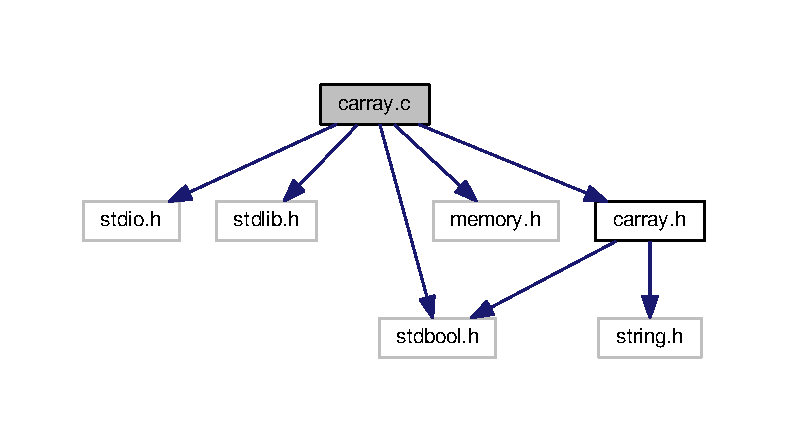
\includegraphics[width=350pt]{carray_8c__incl}
\end{center}
\end{figure}
\subsection*{Functions}
\begin{DoxyCompactItemize}
\item 
void {\bf fatal\+\_\+error} (char message[$\,$])
\item 
{\bf carray} $\ast$ {\bf carray\+\_\+new} ()
\item 
{\bf carray} $\ast$ {\bf carray\+\_\+new\+\_\+\+I\+SC} (size\+\_\+t init\+\_\+space)
\item 
{\bf carray} $\ast$ {\bf carray\+\_\+new\+\_\+\+CC} ({\bf carray} $\ast$copy\+\_\+carray)
\item 
{\bf carray} $\ast$ {\bf carray\+\_\+new\+\_\+\+C\+I\+SC} ({\bf carray} $\ast$copy\+\_\+carray, size\+\_\+t init\+\_\+space)
\item 
void {\bf carray\+\_\+free} ({\bf carray} $\ast$c, void($\ast$voidfunc)(type))
\item 
size\+\_\+t {\bf carray\+\_\+getsize} ({\bf carray} $\ast$c)
\item 
size\+\_\+t {\bf carray\+\_\+getspace} ({\bf carray} $\ast$c)
\item 
void {\bf carray\+\_\+setspace} ({\bf carray} $\ast$c, size\+\_\+t new\+\_\+space, void $\ast$$\ast$ok)
\item 
void {\bf carray\+\_\+addspace} ({\bf carray} $\ast$c, void $\ast$$\ast$ok)
\item 
void {\bf carray\+\_\+safeset} ({\bf carray} $\ast$c, int index, type value, void $\ast$$\ast$ok)
\item 
void {\bf carray\+\_\+append} ({\bf carray} $\ast$c, {\bf carray} $\ast$o, void $\ast$$\ast$ok)
\item 
size\+\_\+t {\bf carray\+\_\+getreadposition} ({\bf carray} $\ast$c)
\item 
void {\bf carray\+\_\+setreadposition} ({\bf carray} $\ast$c, int new\+\_\+read\+\_\+position, void $\ast$$\ast$ok)
\item 
size\+\_\+t {\bf carray\+\_\+readingsremaining} ({\bf carray} $\ast$c)
\item 
type $\ast$ {\bf carray\+\_\+getarray} ({\bf carray} $\ast$c)
\item 
type {\bf carray\+\_\+read} ({\bf carray} $\ast$c, void $\ast$$\ast$ok)
\item 
void {\bf carray\+\_\+push} ({\bf carray} $\ast$c, type value)
\item 
void {\bf carray\+\_\+ins} ({\bf carray} $\ast$c, type value)
\item 
type {\bf carray\+\_\+pop} ({\bf carray} $\ast$c)
\item 
void {\bf carray\+\_\+adjust} ({\bf carray} $\ast$c, void $\ast$$\ast$ok)
\item 
void {\bf carray\+\_\+reverse} ({\bf carray} $\ast$c)
\item 
{\bf carray} $\ast$ {\bf carray\+\_\+reversed\+\_\+\+TF} ({\bf carray} $\ast$c)
\item 
{\bf carray} $\ast$ {\bf carray\+\_\+concat\+\_\+\+TF} ({\bf carray} $\ast$a, {\bf carray} $\ast$b)
\item 
hashtype {\bf carray\+\_\+hashcode} ({\bf carray} $\ast$c, hashtype($\ast$hashfunc)(type))
\item 
bool {\bf carray\+\_\+equal} ({\bf carray} $\ast$a, {\bf carray} $\ast$b, bool($\ast$eqfunc)(type, type))
\item 
char $\ast$ {\bf carray\+\_\+tostring\+\_\+\+TF} ({\bf carray} $\ast$c, char $\ast$($\ast$strfunc)(type), char $\ast$opener, char $\ast$closer, char $\ast$prefix, char $\ast$suffix)
\item 
bool {\bf carray\+\_\+isempty} ({\bf carray} $\ast$c)
\item 
bool {\bf carray\+\_\+contains} ({\bf carray} $\ast$c, type test\+\_\+element, bool($\ast$eqfunc)(type, type))
\item 
type $\ast$ {\bf carray\+\_\+toarray\+\_\+\+TF} ({\bf carray} $\ast$c)
\item 
bool {\bf carray\+\_\+remove\+\_\+elt} ({\bf carray} $\ast$c, type test\+\_\+element, bool($\ast$eqfunc)(type, type))
\item 
void {\bf carray\+\_\+clear} ({\bf carray} $\ast$c)
\item 
type {\bf carray\+\_\+get} ({\bf carray} $\ast$c, int index, void $\ast$$\ast$ok)
\item 
void {\bf carray\+\_\+set} ({\bf carray} $\ast$c, int index, type new\+\_\+value, void $\ast$$\ast$ok)
\item 
void {\bf carray\+\_\+add} ({\bf carray} $\ast$c, int index, type new\+\_\+value, void $\ast$$\ast$ok)
\item 
type {\bf carray\+\_\+remove} ({\bf carray} $\ast$c, int index, void $\ast$$\ast$ok)
\item 
int {\bf carray\+\_\+indexof} ({\bf carray} $\ast$c, type test\+\_\+value, bool($\ast$eqfunc)(type, type))
\item 
int {\bf carray\+\_\+lastindexof} ({\bf carray} $\ast$c, type test\+\_\+value, bool($\ast$eqfunc)(type, type))
\item 
{\bf carray} $\ast$ {\bf carray\+\_\+subcarray\+\_\+\+TF} ({\bf carray} $\ast$c, int from\+\_\+index, int to\+\_\+index, void $\ast$$\ast$ok)
\item 
{\bf carray} $\ast$ {\bf carray\+\_\+subcarraystep\+\_\+\+TF} ({\bf carray} $\ast$c, int from\+\_\+index, int to\+\_\+index, int step, void $\ast$$\ast$ok)
\item 
type $\ast$ {\bf carray\+\_\+subarray\+\_\+\+TF} ({\bf carray} $\ast$c, int from\+\_\+index, int to\+\_\+index, void $\ast$$\ast$ok)
\item 
type $\ast$ {\bf carray\+\_\+subarraystep\+\_\+\+TF} ({\bf carray} $\ast$c, int from\+\_\+index, int to\+\_\+index, int step, void $\ast$$\ast$ok)
\item 
void {\bf carray\+\_\+free\+\_\+obj} (type val)
\end{DoxyCompactItemize}


\subsection{Detailed Description}
Implementation of the carray class. Contains all the function implementations and documentation. 


\section{carray.\+h File Reference}
\label{carray_8h}\index{carray.\+h@{carray.\+h}}


Header of the carray class. Contains all function declarations and preprocessor directives.  


{\ttfamily \#include $<$stdbool.\+h$>$}\\*
{\ttfamily \#include $<$string.\+h$>$}\\*
Include dependency graph for carray.\+h\+:\nopagebreak
\begin{figure}[H]
\begin{center}
\leavevmode
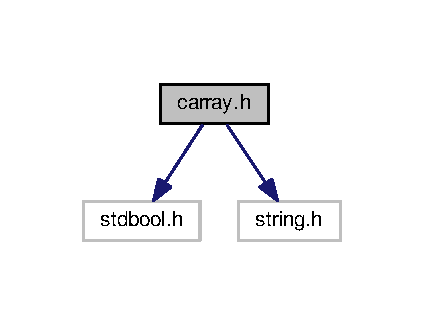
\includegraphics[width=204pt]{carray_8h__incl}
\end{center}
\end{figure}
This graph shows which files directly or indirectly include this file\+:\nopagebreak
\begin{figure}[H]
\begin{center}
\leavevmode
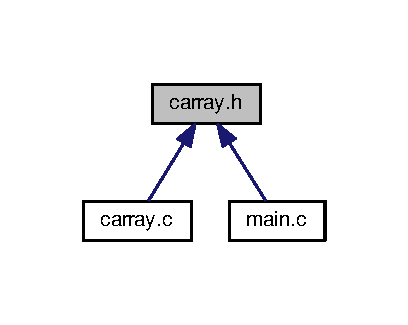
\includegraphics[width=196pt]{carray_8h__dep__incl}
\end{center}
\end{figure}
\subsection*{Data Structures}
\begin{DoxyCompactItemize}
\item 
struct {\bf carray}
\end{DoxyCompactItemize}
\subsection*{Macros}
\begin{DoxyCompactItemize}
\item 
\#define {\bf D\+E\+F\+A\+U\+L\+T\+\_\+\+S\+P\+A\+C\+E\+\_\+\+I\+N\+I\+T\+\_\+\+F\+L\+AT}~8
\item 
\#define {\bf D\+E\+F\+A\+U\+L\+T\+\_\+\+S\+P\+A\+C\+E\+\_\+\+I\+N\+I\+T\+\_\+\+P\+E\+R\+C\+E\+NT}~1.\+25
\item 
\#define {\bf D\+E\+F\+A\+U\+L\+T\+\_\+\+S\+P\+A\+C\+E\+\_\+\+I\+N\+CR}~2.\+0
\item 
\#define {\bf D\+E\+F\+A\+U\+L\+T\+\_\+\+S\+H\+R\+I\+N\+K\+\_\+\+T\+H\+R\+E\+S\+H\+O\+LD}~2.\+5
\item 
\#define {\bf D\+E\+F\+A\+U\+L\+T\+\_\+\+S\+H\+R\+I\+N\+K\+\_\+\+P\+E\+R\+C\+E\+NT}~1.\+25
\item 
\#define {\bfseries P\+R\+I\+M\+E\+\_\+\+C\+ST}~31
\item 
\#define {\bfseries D\+E\+F\+A\+U\+L\+T\+\_\+\+T\+Y\+P\+E\+\_\+\+V\+A\+L\+UE}~N\+U\+LL
\item 
\#define {\bfseries of\+\_\+\+Char}~$\ast$(char$\ast$)
\item 
\#define {\bfseries of\+\_\+s\+Char}~$\ast$(signed char$\ast$)
\item 
\#define {\bfseries of\+\_\+u\+Char}~$\ast$(unsigned char$\ast$)
\item 
\#define {\bfseries of\+\_\+\+Short}~$\ast$(short$\ast$)
\item 
\#define {\bfseries of\+\_\+s\+Short}~$\ast$(signed short$\ast$)
\item 
\#define {\bfseries of\+\_\+u\+Short}~$\ast$(unsigned short$\ast$)
\item 
\#define {\bfseries of\+\_\+\+Int}~$\ast$(int$\ast$)
\item 
\#define {\bfseries of\+\_\+s\+Int}~$\ast$(signed int$\ast$)
\item 
\#define {\bfseries of\+\_\+u\+Int}~$\ast$(unsigned int$\ast$)
\item 
\#define {\bfseries of\+\_\+\+Long}~$\ast$(long$\ast$)
\item 
\#define {\bfseries of\+\_\+l\+Long}~$\ast$(long long$\ast$)
\item 
\#define {\bfseries of\+\_\+s\+Long}~$\ast$(signed long$\ast$)
\item 
\#define {\bfseries of\+\_\+sl\+Long}~$\ast$(signed long long$\ast$)
\item 
\#define {\bfseries of\+\_\+u\+Long}~$\ast$(unsigned long$\ast$)
\item 
\#define {\bfseries of\+\_\+ul\+Long}~$\ast$(unsigned long long$\ast$)
\item 
\#define {\bfseries of\+\_\+\+Float}~$\ast$(float$\ast$)
\item 
\#define {\bfseries of\+\_\+\+Double}~$\ast$(double$\ast$)
\item 
\#define {\bfseries of\+\_\+l\+Double}~$\ast$(long double$\ast$)
\item 
\#define {\bfseries of\+\_\+\+Bool}~$\ast$(bool$\ast$)
\item 
\#define {\bfseries of\+\_\+\+String}~(char$\ast$)
\item 
\#define {\bfseries Char}(expr)
\item 
\#define {\bfseries s\+Char}(expr)
\item 
\#define {\bfseries u\+Char}(expr)
\item 
\#define {\bfseries Short}(expr)
\item 
\#define {\bfseries s\+Short}(expr)
\item 
\#define {\bfseries u\+Short}(expr)
\item 
\#define {\bfseries Int}(expr)
\item 
\#define {\bfseries s\+Int}(expr)
\item 
\#define {\bfseries u\+Int}(expr)
\item 
\#define {\bfseries Long}(expr)
\item 
\#define {\bfseries l\+Long}(expr)
\item 
\#define {\bfseries s\+Long}(expr)
\item 
\#define {\bfseries sl\+Long}(expr)
\item 
\#define {\bfseries u\+Long}(expr)
\item 
\#define {\bfseries ul\+Long}(expr)
\item 
\#define {\bfseries Float}(expr)
\item 
\#define {\bfseries Double}(expr)
\item 
\#define {\bfseries l\+Double}(expr)
\item 
\#define {\bfseries Bool}(expr)
\item 
\#define {\bfseries String}(expr)
\item 
\#define {\bfseries free\+\_\+\+Obj}~\&{\bf carray\+\_\+free\+\_\+obj}
\end{DoxyCompactItemize}
\subsection*{Typedefs}
\begin{DoxyCompactItemize}
\item 
typedef struct {\bf carray} {\bf carray}
\item 
typedef unsigned int {\bfseries hashtype}
\item 
typedef void $\ast$ {\bfseries type}
\end{DoxyCompactItemize}
\subsection*{Functions}
\begin{DoxyCompactItemize}
\item 
void {\bf carray\+\_\+free\+\_\+obj} (type)
\item 
{\bf carray} $\ast$ {\bf carray\+\_\+new} ()
\item 
{\bf carray} $\ast$ {\bf carray\+\_\+new\+\_\+\+I\+SC} (size\+\_\+t)
\item 
{\bf carray} $\ast$ {\bf carray\+\_\+new\+\_\+\+CC} ({\bf carray} $\ast$)
\item 
{\bf carray} $\ast$ {\bf carray\+\_\+new\+\_\+\+C\+I\+SC} ({\bf carray} $\ast$, size\+\_\+t)
\item 
void {\bfseries carray\+\_\+free} ({\bf carray} $\ast$, void(type))
\item 
size\+\_\+t {\bf carray\+\_\+getsize} ({\bf carray} $\ast$)
\item 
void {\bf carray\+\_\+clear} ({\bf carray} $\ast$)
\item 
bool {\bf carray\+\_\+isempty} ({\bf carray} $\ast$)
\item 
size\+\_\+t {\bf carray\+\_\+getspace} ({\bf carray} $\ast$)
\item 
void {\bf carray\+\_\+setspace} ({\bf carray} $\ast$, size\+\_\+t, void $\ast$$\ast$)
\item 
void {\bf carray\+\_\+adjust} ({\bf carray} $\ast$, void $\ast$$\ast$)
\item 
size\+\_\+t {\bf carray\+\_\+getreadposition} ({\bf carray} $\ast$)
\item 
size\+\_\+t {\bf carray\+\_\+readingsremaining} ({\bf carray} $\ast$)
\item 
void {\bf carray\+\_\+setreadposition} ({\bf carray} $\ast$, int, void $\ast$$\ast$)
\item 
type $\ast$ {\bf carray\+\_\+getarray} ({\bf carray} $\ast$)
\item 
type {\bf carray\+\_\+read} ({\bf carray} $\ast$, void $\ast$$\ast$ok)
\item 
void {\bf carray\+\_\+reverse} ({\bf carray} $\ast$)
\item 
{\bf carray} $\ast$ {\bf carray\+\_\+reversed\+\_\+\+TF} ({\bf carray} $\ast$)
\item 
void {\bf carray\+\_\+append} ({\bf carray} $\ast$, {\bf carray} $\ast$, void $\ast$$\ast$)
\item 
{\bf carray} $\ast$ {\bf carray\+\_\+concat\+\_\+\+TF} ({\bf carray} $\ast$, {\bf carray} $\ast$)
\item 
char $\ast$ {\bfseries carray\+\_\+tostring\+\_\+\+TF} ({\bf carray} $\ast$, char $\ast$(type), char $\ast$, char $\ast$, char $\ast$, char $\ast$)
\item 
hashtype {\bfseries carray\+\_\+hashcode} ({\bf carray} $\ast$, hashtype(type))
\item 
bool {\bfseries carray\+\_\+equal} ({\bf carray} $\ast$, {\bf carray} $\ast$, bool(type, type))
\item 
int {\bfseries carray\+\_\+indexof} ({\bf carray} $\ast$, type, bool(type, type))
\item 
int {\bfseries carray\+\_\+lastindexof} ({\bf carray} $\ast$, type, bool(type, type))
\item 
bool {\bfseries carray\+\_\+contains} ({\bf carray} $\ast$, type, bool(type, type))
\item 
{\bf carray} $\ast$ {\bf carray\+\_\+subcarray\+\_\+\+TF} ({\bf carray} $\ast$, int, int, void $\ast$$\ast$)
\item 
{\bf carray} $\ast$ {\bf carray\+\_\+subcarraystep\+\_\+\+TF} ({\bf carray} $\ast$, int, int, int, void $\ast$$\ast$)
\item 
type $\ast$ {\bf carray\+\_\+subarray\+\_\+\+TF} ({\bf carray} $\ast$, int, int, void $\ast$$\ast$)
\item 
type $\ast$ {\bf carray\+\_\+subarraystep\+\_\+\+TF} ({\bf carray} $\ast$, int, int, int, void $\ast$$\ast$)
\item 
type $\ast$ {\bf carray\+\_\+toarray\+\_\+\+TF} ({\bf carray} $\ast$)
\item 
type {\bf carray\+\_\+get} ({\bf carray} $\ast$, int, void $\ast$$\ast$)
\item 
void {\bf carray\+\_\+add} ({\bf carray} $\ast$, int, type, void $\ast$$\ast$)
\item 
void {\bf carray\+\_\+push} ({\bf carray} $\ast$, type)
\item 
void {\bf carray\+\_\+ins} ({\bf carray} $\ast$, type)
\item 
void {\bf carray\+\_\+set} ({\bf carray} $\ast$, int, type, void $\ast$$\ast$)
\item 
void {\bf carray\+\_\+safeset} ({\bf carray} $\ast$, int, type, void $\ast$$\ast$)
\item 
type {\bf carray\+\_\+remove} ({\bf carray} $\ast$, int, void $\ast$$\ast$)
\item 
type {\bf carray\+\_\+pop} ({\bf carray} $\ast$)
\item 
bool {\bfseries carray\+\_\+remove\+\_\+elt} ({\bf carray} $\ast$, type, bool(type, type))
\end{DoxyCompactItemize}
\subsection*{Variables}
\begin{DoxyCompactItemize}
\item 
char $\ast$ {\bfseries Char\+\_\+holder}
\item 
signed char $\ast$ {\bfseries s\+Char\+\_\+holder}
\item 
unsigned char $\ast$ {\bfseries u\+Char\+\_\+holder}
\item 
short $\ast$ {\bfseries Short\+\_\+holder}
\item 
signed short $\ast$ {\bfseries s\+Short\+\_\+holder}
\item 
unsigned short $\ast$ {\bfseries u\+Short\+\_\+holder}
\item 
int $\ast$ {\bfseries Int\+\_\+holder}
\item 
signed int $\ast$ {\bfseries s\+Int\+\_\+holder}
\item 
unsigned int $\ast$ {\bfseries u\+Int\+\_\+holder}
\item 
long $\ast$ {\bfseries Long\+\_\+holder}
\item 
long long $\ast$ {\bfseries l\+Long\+\_\+holder}
\item 
signed long $\ast$ {\bfseries s\+Long\+\_\+holder}
\item 
signed long long $\ast$ {\bfseries sl\+Long\+\_\+holder}
\item 
unsigned long $\ast$ {\bfseries u\+Long\+\_\+holder}
\item 
unsigned long long $\ast$ {\bfseries ul\+Long\+\_\+holder}
\item 
float $\ast$ {\bfseries Float\+\_\+holder}
\item 
double $\ast$ {\bfseries Double\+\_\+holder}
\item 
long double $\ast$ {\bfseries l\+Double\+\_\+holder}
\item 
bool $\ast$ {\bfseries Bool\+\_\+holder}
\item 
char $\ast$ {\bfseries String\+\_\+holder}
\end{DoxyCompactItemize}


\subsection{Detailed Description}
Header of the carray class. Contains all function declarations and preprocessor directives. 


%--- End generated contents ---

% Index
\backmatter
\newpage
\phantomsection
\clearemptydoublepage
\addcontentsline{toc}{chapter}{Index}
\printindex

\end{document}
